% =============================================================================
% paper/ko/main.tex — 한국어 보조 원고 (KAEA 학회 발표 + 학위논문 chapter 기반)
%
% Title:   농가별 정액 직불제 컷오프에서 농가모형 분리성 검정: 한국의 증거
% Author:  이도현 (고려대학교 식품자원경제학과)
% Status:  Wave 10.5 KO 재유도 (2026-05-20) — paper/en (Wave 10.5) 전면 미러
%
% 컴파일:  cd paper/ko && latexmk -xelatex -interaction=nonstopmode main.tex
% Bib:     ../../Bibliography_base.bib (27 entries; plainnat 영문식 출력)
%
% Plan:    quality_reports/plans/velvet-frolicking-glade.md
% Note:    paper/ko는 paper/en에서 파생 — 정합성 유지 필수.
%          영문 저자 인용은 \citet{} 그대로 사용 (plainnat 양쪽 동일 출력 검증됨).
%          한국 저자 인용 (ChoiMun2025, KAMICO_pricelist_2022)은 본문 수동 인라인.
% =============================================================================

\documentclass[12pt, a4paper]{article}
% =============================================================================
% paper/ko/preamble_ko.tex — XeLaTeX preamble for the Korean derived paper.
%
% Mirrors paper/en/preamble_en.tex with kotex added for Korean text rendering.
% Used by KAEA / 한국농경제학회 conference presentation + future thesis chapter.
%
% paper/ko derives from paper/en post-stabilization (CLAUDE.md project convention);
% user authorized 2026-05-15 to create alongside paper/en in this session.
% =============================================================================

% Engine detection + encoding (pdfTeX fallback)
\usepackage{iftex}
\ifPDFTeX
  \usepackage[utf8]{inputenc}
\fi

% Korean rendering (kotex auto-loads fontspec under XeLaTeX)
\usepackage{kotex}

% Math + tables + graphics
\usepackage{amsmath, amssymb, amsthm}
\usepackage{booktabs}
\usepackage{graphicx}
\usepackage{caption}
\captionsetup{font=small, labelfont=bf}

% Page geometry (1in margins, A4)
\usepackage[a4paper, margin=1in]{geometry}

% Double-spacing for journal submission
\usepackage{setspace}
\doublespacing

% Palette (mirrors Quarto/theme-template.scss; consistent with Preambles/header.tex)
\usepackage{xcolor}
\definecolor{primary-blue}{HTML}{012169}
\definecolor{primary-gold}{HTML}{B9975B}
\definecolor{highlight-yellow}{HTML}{F2A900}
\definecolor{light-bg}{HTML}{E8EDF5}
\definecolor{jet}{HTML}{1A1A1A}
\definecolor{positive}{HTML}{15803D}
\definecolor{negative}{HTML}{B91C1C}
\definecolor{neutral}{HTML}{525252}
\colorlet{accent}{primary-blue}
\colorlet{accent2}{primary-gold}

% Hyperref (loaded after xcolor so link colors resolve)
% unicode=true required for Korean bookmarks/TOC under XeLaTeX + kotex
\usepackage[unicode]{hyperref}
\hypersetup{
  colorlinks = true,
  linkcolor  = primary-blue,
  urlcolor   = primary-blue,
  citecolor  = primary-blue,
  pdfborder  = {0 0 0}
}

% Citation engine — author-year style.
% Korean-authored entries use Korean form by directory convention; English-authored
% entries (all 11 current §3 cites) use English author-year regardless of paper lang.
\usepackage[round, authoryear]{natbib}
\bibliographystyle{plainnat}

% Convenience macros (re-used from Preambles/header.tex)
\newcommand{\muted}[1]{\textcolor{neutral}{#1}}
\newcommand{\key}[1]{\textcolor{primary-gold}{\textbf{#1}}}
\newcommand{\good}[1]{\textcolor{positive}{#1}}
\newcommand{\bad}[1]{\textcolor{negative}{#1}}

% Section-numbering depth
\setcounter{secnumdepth}{3}
\setcounter{tocdepth}{2}

% Theorem-like environments (예측 = numbered claim by channel)
\theoremstyle{plain}
\newtheorem{prediction}{예측}[section]


\title{농가별 정액 직불제 컷오프에서 농가모형 분리성 검정:\\
       한국의 증거}
\author{이도현\\
        고려대학교\\
        식품자원경제학과}
\date{초안: \today}

\begin{document}
\maketitle

\begin{abstract}
\noindent
한국의 2020년 공익직불제(PIDPS)는 미국 및 EU 공동농업정책(CAP)의 면적비례 설계와 달리, 0.5\,ha 경지면적 컷오프 이하 소농에게 연 120만원을 \emph{농가별 정액}으로 지급한다 \citep{Kirwan2009_rentcap, BaldoniCiaian2023_eucap}. 본 논문은 농가경제조사(FHES) 패널($N = 11{,}010$ 농가-연도, $2{,}776$ 농가, 2018--2022년)에 대해 이중차분-회귀불연속(DiD-RD) 설계를 적용하여 이 컷오프에서 농가모형(AHM)의 분리성 귀무가설을 검정한다. 양쪽 면에 관측가능한 자격 스크리닝을 대칭적으로 적용한다. AHM의 두 확장은 검증 가능한 예측을 제공한다. 자산편향 유동성 \citep{CarterOlinto2003_liquidity}은 임차에 대한 단조감소 구배를 자작 면적에 예측한다(F1, 일차); 암묵노동-감독 \citep{EswaranKotwal1986_supervision}은 고용노동 마진의 반응을 예측한다(F2, 보조).

순임차 농가의 자작면적 반응은 T2 대역폭에서 $+1{,}151$\,m\textsuperscript{2}이며($p = .036$), 4개 비-순소유 구간에 걸쳐 단조감소한다($+1{,}151 \to +438 \to +258 \to -52 \to 0$). 농가별 정액 설계는 면적비례 일정에서 관찰된 임차료 전가를 \emph{반전}시킨다: 임차료 전가는 T1에서 $-13.7\%$($p < .10$)이며, 미국의 $+25\%$ \citep{Kirwan2009_rentcap} 및 EU의 $+46$--$55\%$ \citep{BaldoniCiaian2023_eucap}와 대조된다. 임차료 차감 농업경영비 반응은 T1에서 $-3.57$\,M\,KRW로 (S,s) 비활동 해석을 지지한다(다중검정 보정 후 개별적으로 유의하지 않음). 자산편향 유동성 채널을 통해 신용제약 비-순소유 부분모집단에 대해 0.5\,ha 컷오프에서 AHM 분리성을 기각한다; 농가별 정액 지급 설계 자체가 면적당 지주 포착 채널을 단절하는 정책 레버리지이다.
\end{abstract}

\noindent\textbf{핵심어:} 농가모형(AHM); 분리성; 회귀불연속; 이중차분; 직불금; 소농; 유동성; 한국.

\noindent\textbf{JEL 분류:} Q12, Q15, Q18, D13, D14.

\bigskip

% =============================================================================
\section{서론}
% =============================================================================
\label{sec:intro}

농가별 정액 직불제의 0.5\,ha 컷오프에서, 한국의 소농에 대해 농가모형의 분리성 귀무가설이 성립하는가? 기각된다면 어떤 메커니즘을 통해 실패하는가? 한국의 2020년 공익직불제(PIDPS)는 20년 만의 최대 직불제 구조개편으로, 면적비례 쌀소득보전직불제를 폐지하고 소농직불금(SFFP)을 농가별 정액 부문으로 포함하는 혼합형 프로그램을 도입했다. SFFP는 기준연도 경지면적이 0.5\,ha($5{,}000$\,m\textsuperscript{2}) 이하인 농가에 연 $1{,}200{,}000$\,KRW를 지급한다.\footnote{2020년 시행 시 금액은 농가당 연 120만원이며 2018--2022년 표본 기간 전체에 동일하게 적용되었다. SFFP는 2025년 130만원으로 인상되었으나, 본 논문의 모든 magnitude는 120만원 기간을 기준으로 해석된다.} 약 100만 농가가 매년 PIDPS 지급을 받으며, 총 예산 2.3조 원 중 SFFP가 약 20\%를 차지한다. 농어업인 등에 대한 공익직불금 지급에 관한 법률 제10조는 ``농가 소득 안정''과 ``농업·농촌 공익기능 증진''의 이중 목표를 명시한다. 농가별 정액 설계는 제도적으로 차별적이다: 미국 작물보조의 면적비례 구조 \citep{Kirwan2009_rentcap}나 EU 공동농업정책 1축 \citep{BaldoniCiaian2023_eucap}과 달리, 가장 가까운 비교 대상은 유사한 국가단위 비-초국가 직불제에 대한 스위스 공간 RD이다 \citep{ZimmertZorn2022_swissrd}.

농가모형(AHM)의 분리성 귀무가설은, 완전시장 하에서 소농의 생산 결정---토지 보유, 자본투자, 노동 배분---이 소비 결정과 재귀적으로 분리 가능하다는 것이다. 따라서 정액 이전소득은 오직 소비 부문에만 들어가고 생산에는 영향을 미치지 않는다 \citep{SinghSquireStrauss1986_ahm, deJanvryFafchampsSadoulet1991_peasant}. 본 논문은 이 귀무가설을 0.5\,ha SFFP 컷오프에서 검정한다. 분리성 검정 문헌 \citep{Benjamin1992_separation, LaFaveThomas2016_markets}은 일반적으로 개발도상국 환경에서 인구통계학적 충격을 도구변수로 사용하여 분리성을 기각해 왔지만, 본 연구는 선진국 정책 컷오프를 활용한다. 본 연구의 틀은 분리성이 실패하는 두 가지 AHM 확장을 형식화한다. \textbf{자산편향 유동성} 채널 \citep{CarterOlinto2003_liquidity}은 일차적 채널(채널 A)이다: 신용 접근성은 기준 부에 따라 증가하며, SFFP 이전소득은 임차 대 자작 마진을 임차율 분포에 걸쳐 비대칭적으로 완화한다. \textbf{암묵노동-감독} 채널 \citep{EswaranKotwal1986_supervision}은 보조적이다(채널 B): 가족노동이 고용노동과 불완전 대체될 때 농가의 잠재임금이 시장임금과 괴리된다. 가격 조정의 협상·임대료 귀착 마진은 농가모형 핵심 외부의 축약형 평형 함의로 분석에 들어오며, \S\ref{sec:discussion}에서 다룬다. 본 범위 내에서 두 가지 위증 트리거를 사전 명시한다: F1은 자작면적에 대한 임차율의 단조 구배(자산편향 채널의 부담-기각 트리거); F2는 농외소득에 대한 고용노동 마진 반응(EK 도출의 부호 비결정성 하에서 기각-부담 아님; 감독 채널에 대한 정보 제공).\footnote{이론적 범위, 결과변수 위계, F1/F2 사전 명세는 추정 이전에 고정되었으며, 해당 사전명세 archive는 재현 패키지에 포함된다.}

본 연구의 기여는 네 가지 기준점에 대해 정의된다. 면적비례 직불금 귀착에 관한 미국·EU 문헌---\citet{Kirwan2009_rentcap}이 기록한 미국 직접·역경기보조금의 약 25\% 임차료 자본화, \citet{BaldoniCiaian2023_eucap}이 보고한 EU 공동농업정책 1축의 $9.1$--$55\%$ 전가---은 면적당 설계 하에서 상당한 지주 임대료 추출의 선진국 사전확률을 확립한다. SFFP의 농가별 정액 설계는 구성상 이 채널을 단절하며, 본 연구의 틀은 임대 귀착을 농가모형 핵심 외부의 축약형 평형 함의로 다룬다. \citet{Kazukauskas2013_disinvestment}의 디커플링 유도 비투자 결과는 영업비 하위예측의 가장 가까운 이론적 계보이다(이전이 덩어리 조정비용에 대해 작을 때 (S,s) 비활동 구간이 깊어지고 영업비가 감소; \citealp{CaballeroEngel1999_lumpy}). 본 연구는 비투자 문헌이 분리하지 않는 자산편향 시그너처(Carter--Olinto 교차편미분)를 형식화하여 이 계보를 확장한다. 이론적 구조에서 가장 가까운 것은 \citet{CarterOlinto2003_liquidity}이며, 파라과이 농촌의 토지 등기 증거를 선진국 직불제 맥락에서 더 정교한 식별로 재현한다. F1과 F2가 모두 발동하지 않는다면, 결합 귀무는 \citet{LaFaveThomas2016_markets}의 정확한 보완---노동·신용시장이 완전성에 접근하는 곳에서 살아남는 소농의 분리성---이 된다.

본 연구는 0.5\,ha SFFP 컷오프를 활용한 이중차분-회귀불연속(DiD-RD) 설계로 처치효과를 식별한다. 처치는 정책 후 조작을 배제하기 위해 2018년 기준연도에서 동결된 $rv_{2018,i} = A_{2018,i} - 5{,}000$\,m\textsuperscript{2}을 실행변수로 한다(\S\ref{sec:institutional-eligibility}). 처치 더미 $D_i$는 FHES 관측 가능한 3개 SFFP 기준의 결합이다; 이 스크리닝을 컷오프 양쪽에 대칭적으로 적용하여 $N = 11{,}010$ 농가-연도, $2{,}776$ 농가의 표본을 얻으며, 스크리닝된 부분모집단에서 $D_i = 1 \iff rv_{2018,i} \le 0$이 성립한다. 추정량은 의도된 처치 효과(intent-to-treat, ITT)이며 sharp ATT는 아니다. 관측 불가능한 5개 기준의 행정적 준수율은 약 92\%이다(\S\ref{sec:institutional-identification}). 완전한 식별 명세---대역폭 그리드(T1/T2/T3), 클러스터-강건 + 와일드 클러스터 부트스트랩 추론, 일차 결과변수 가족에 걸친 Holm step-down---는 \S\ref{sec:identification}에 제시된다. 일차 결과변수는 자작면적($A_{\text{own}}$)과 임차료 차감 농업경영비(op\_cost\_ex\_rent)이며; 보조 결과변수는 농외소득(F2 감독-마진 진단)이다.

F1은 $\partial A_{\text{own},i} / \partial T_{SFFP}$에 대해 기준 임차율의 단조 구배를 예측한다: 가장 낮은 기준 자작비율을 가진 순임차 소농이 가장 큰 반응을 보이며; $s_0 = 1$에 고정된 순소유 소농은 구성상 0 반응을 보인다(\S\ref{sec:liquidity}에서 $s_0 = A_{\text{own},2018}/A_{2018}$에 대한 5분위 분할이 사전 명시됨). 이전-조정비용 비율 $T_{SFFP}/\tau \in [0.024, 0.048]$(\S\ref{sec:calibration})은 \citet{CaballeroEngel1999_lumpy} 유형 모형의 (S,s) 비활동 구간 내에 코호트를 위치시키며, 영업비 하위예측 $\beta_{\text{op\_cost\_ex\_rent}} \le 0$을 지지한다. \S\ref{sec:results}의 추정치는 F1 단조 임차율 구배를 확인하며(순임차 자작면적 반응 T2에서 $+1{,}151$\,m\textsuperscript{2}, $p = .036$; 저소유 $+438$\,m\textsuperscript{2}, $p = .047$), T1에서 $-3.57$\,M\,KRW의 임차료 차감 영업비 반응은 (S,s) 해석을 지지한다. 임차료 전가의 축약형은 T1에서 $-13.7\%$($p < .10$)로, 미국($+25\%$, \citealp{Kirwan2009_rentcap})과 EU 공동농업정책($+46$--$55\%$, \citealp{BaldoniCiaian2023_eucap}) 벤치마크와 정반대 부호이다.

본 논문은 세 가지 기여를 한다. \emph{방법론적으로}, 본 연구는 농가별 정액 직불금 컷오프에서 최초의 AHM 분리성 검정이며, 한국 PIDPS에 대한 최초의 DiD-RD 증거를 제공한다. 컷오프 설계는 공간적 자격 불연속을 시간적 정책 개혁과 결합함으로써 기존 한국 직불금 연구를 확장한다. 추가로, 면적 컷오프 단독에 의존하지 않고 3개 FHES 관측가능한 법정 기준의 결합에 대해 ITT를 추정함으로써 정책 정의에 경험적 처치 지표를 일치시키며, 면적 자격이지만 법정 비자격인 14.6\% 마진을 별도로 기록한다(\S\ref{sec:robustness-areaonly}는 면적 단독 처치 강건성 비교를 보고한다). \citet{ChoiJodlowski2025_landreg}는 한국의 토지소유권 규제를 연구하지만 컷오프에서의 SFFP 보조금은 다루지 않는다; 최민영·문한필(2025)은 동일한 0.5\,ha 임계값에서 농외소득 RDD를 적용하지만, AHM 분리성 검정과 DiD-RD 설계를 결합하지 않는다 \citep{ChoiMun2025_pidps_offinc}. \emph{이론적으로}, 두 개의 비분리성(자산편향 유동성, 암묵노동-감독)을 가진 AHM 확장 틀을 제공하며, 임대 귀착 마진에 대한 명시적 이론 외 공개(\S\ref{sec:theory} 평형-임대료 caveat)와 함께 닫힌 형태의 위증 가능한 예측을 산출한다. \emph{경험적으로}, 자작면적의 단조 임차율 구배와 (S,s) 영업비 반응은 농가별 정액 설계가 Kirwan--Baldoni-Ciaian 자본화 채널을 약화시키는 소농 환경에서 비-귀착-마진 직불금 효과에 관한 선진국 증거를 제공한다.

본 논문의 나머지는 다음과 같이 구성된다. \S\ref{sec:institutional}은 제도적 맥락을 상세히 다룬다. \S\ref{sec:theory}는 개념적 틀을 발전시킨다. \S\ref{sec:data}는 자료를 기술한다. \S\ref{sec:identification}은 식별 전략을 명시한다. \S\ref{sec:results}는 헤드라인 결과를 보고한다. \S\ref{sec:robustness}는 강건성 검정을 수행한다. \S\ref{sec:discussion}은 정책적·이론적 함의를 논의하고 결론을 맺는다.

% =============================================================================
\section{제도적 배경}
% =============================================================================
\label{sec:institutional}

\subsection{2020년 공익직불제 개혁과 2분기 일정}
\label{sec:institutional-reform}

2020년 5월 1일 시행된 공익직불제(PIDPS)는 농어업인 등에 대한 공익직불금 지급에 관한 법률 제10조에 따라, 2000년대와 2010년대에 축적된 쌀소득보전직불제와 일련의 보완적 직불 프로그램들을 하나의 2분기 설계로 통합했다. 두 분기는 농가 수준에서 상호배타적이다: SFFP 자격 농가는 면적직불금(ABP)을 받지 않으며 그 반대도 마찬가지이다. 소농직불금(SFFP)은 경지면적, 작물 선택, 산출과 무관하게 \S\ref{sec:institutional-eligibility}에 기술된 8개 자격 요건을 충족하는 농가에 농가당 연 $1{,}200{,}000$\,KRW를 지급한다. SFFP 자격이 없는 농가에 적용되는 면적직불금(ABP)은 농업 유형 계층별로 다른 ha당 금액을 지급한다: 보호구역 논벼는 ha당 $2{,}050{,}000$\,KRW, 비보호구역 논과 밭은 ha당 $1{,}970{,}000$\,KRW, 한계지 계층은 ha당 $1{,}890{,}000$\,KRW이다.\footnote{지리적 보호지정은 농림축산식품부 고시 2020-23호를 따르며, 본 표본 기간 전체에 안정적으로 유지된다.} 0.5\,ha 컷오프에서 한계 SFFP 자격 농가는 정액 $1{,}200{,}000$\,KRW를 받는다. 컷오프 바로 위(면적 $> 0.5$\,ha)의 농가에 대한 ABP의 반사실적 이전소득은 약 $985{,}000$\,KRW이며(ha당 $1{,}970{,}000$\,KRW 기본요율을 $0.5$\,ha에 적용), 컷오프에서 연 약 $215{,}000$\,KRW의 불연속 기대-이전 점프를 산출한다.

\subsection{SFFP 자격 요건과 관측 가능한 준수}
\label{sec:institutional-eligibility}

SFFP 자격은 농가가 결합으로 충족해야 하는 8개 요건에 조건적이다: (i) 총 경지면적이 0.5\,ha 이하; (ii) 농가-합산 자작 농지가 1.55\,ha 미만; (iii) 세대주의 영농 경력 3년 이상; (iv) 농촌 거주 경력 3년 이상; (v) 개별 농외소득 연 2,000만원 미만(세대원 단위 평가); (vi) 총 농가 농외소득 연 4,500만원 미만(세대원 합산); (vii) 농산물품질관리원(NAQS) 농업경영체 등록; (viii) 토양 관리, 수질, 농약 공시, 생물다양성을 다루는 17개 공익 의무 준수. (viii) 미준수는 농가를 자격에서 배제하는 대신 지급액을 10\% 감액한다. (ii)와 (vi)에 적용되는 농가 정의 규칙은 배우자, 19세 미만 미혼자녀, 그리고 지난 3년 이내 농가를 떠난 자녀를 합산한다---이는 가족 내 분리 회피 조항을 통해 분리 노출 허점을 차단한다.

이 8개 요건 중 0.5\,ha 컷오프 (i)만이 연속적이고 2020년 이전에 고정된 관측치---통계청 농가경제조사(FHES) 2018년 기준 경지면적---에 묶인 sharp 임계값이다. 요건 (ii)(자작면적 1.55\,ha 미만)는 농가-합산 규칙에 따라 토지 등기부를 재집계한 후 FHES에서 관측 가능하며, 요건 (vi)(총 농가 농외소득)는 FHES 소득 모듈에서 직접 관측 가능하다. 요건 (iii)--(v), (vii), (viii)은 농림축산식품부 지역사무소 기록, NAQS 등기부, 한국농수산식품유통공사(aT) 지급 감사를 통해 행정적으로 관리되며, 조사 자료에는 존재하지 않는다.

본 연구의 처치 코호트---2018년 기준 경지면적이 0.5\,ha 이하인 1,325개 농가---내에서 1,131개(85.4\%)는 FHES 관측 가능한 요건 (ii)와 (vi)도 충족하며; 나머지 194개(14.6\%)는 이 두 요건 중 하나에 미달한다. 자작면적 상한 (ii)는 처치 코호트의 1.8\%에서 구속력을 가지며, 농외소득 상한 (vi)는 12.8\%에서 구속력을 가진다.\footnote{12.8\% 농외소득 마진은 한 명 이상의 세대원이 공식 농외 고용에 있고 연간 노동소득만으로 4,500만원 상한에 근접하는 농가에 집중되어 있다.} 14.6\% 미준수 수치는 컷오프에서의 실제 미수령에 대한 보수적 하한이다: 관측 불가능한 요건 (iii)--(v), (vii), (viii)에서 발생할 손실은 누락된다. 따라서 컷오프에서의 행정적 수령은 1보다 의미 있게 낮다.

\subsection{식별 자세와 농가별 정액 레버리지}
\label{sec:institutional-identification}

본 논문은 \S\ref{sec:identification}의 DiD-RD 추정량을 대칭 스크리닝 표본에 대한 의도된 처치 효과(ITT)로 틀짓는다. 0.5\,ha 컷오프는 자격 일정에서 유일한 정책-정의 sharp 임계값이며, 2018년 기준 경지면적은 구성상 조작 방지이다---농가는 2018년 토지를 배분할 때 2020년 5월 개혁을 예상하지 않았다. 주 분석은 컷오프 양쪽에 동일한 (ii)+(vi) 관측가능 자격 스크리닝을 적용하여(\S\ref{sec:identification}), $2{,}776$ 농가의 표본을 산출하며 $D_i = 1 \iff rv_{2018,i} \le 0$이 성립한다. 비대칭 표본 변형(처치 측만 스크리닝하여 194개 처치-비자격 농가를 제외)은 \S\ref{sec:robustness-asymmetric}에서 강건성 검정으로 보고되며; 면적 단독 설계(관측가능 스크리닝 없음)는 \S\ref{sec:robustness-areaonly}에서 보고된다. 두 대안 표본 모두 $A_{\text{own}}$에 대한 F1 단조 구배 부호와 임차료 차감 영업비 반응의 방향을 보존한다. 관측 불가능한 요건 (iii)--(v), (vii), (viii)이 행정적으로 집행되고 조사 자료에 존재하지 않으므로 sharp ATT는 추정하지 않으며; ITT는 스크리닝된 자격 모집단 내 행정적 미수령에 대해 적분한다.

농가별 정액 SFFP 설계는 미국·EU 직불금 문헌 대비 식별 레버리지의 중심적 제도적 원천이다. \citet{Kirwan2009_rentcap}은 미국 직접·역경기보조금의 약 25\%가 농지 임대료에 자본화된다는 점을 기록하며, 이는 미국 지급 일정의 면적당 설계가 추동하는 귀착 결과이다. \citet{BaldoniCiaian2023_eucap}은 EU 공동농업정책 1축 지급의 임대료율 전가가 단기 9.1--46.2\%, 장기 11--55\%라고 보고하며, 마찬가지로 ha당 구조에 의해 추동된다. SFFP는 이러한 설계에서 이탈한다: 농가는 100\,m\textsuperscript{2}을 경작하든 $4{,}900$\,m\textsuperscript{2}을 경작하든 동일한 120만원 정액을 받으며, 면적당 자본화 채널을 구성상 제거한다. \S\ref{sec:robustness}의 T2 대역폭에서 $-12.0\%$ 임차료 전가 추정치는 이 채널의 부재와 제도적으로 일치한다; 농가 반응의 잔여 마진---자산편향 유동성(\S\ref{sec:theory} 채널 A)과 암묵노동-감독(\S\ref{sec:theory} 채널 B)---이 AHM 분리성 검정의 초점이다.

프로그램 규칙과 예산 배분에 대한 자료는 농림축산식품부 행정 기록에서 오며, 자격 확인과 농업경영체 등록은 NAQS에서, SFFP 지급 기록은 한국농수산식품유통공사(aT)에서 유지된다. 본 연구의 분석 자료인 통계청 FHES는 이러한 행정 자료원과 독립적이다; \S\ref{sec:data}에서 FHES 표본을 기술한다.

% =============================================================================
\section{개념적 틀}
% =============================================================================
\label{sec:theory}

% -----------------------------------------------------------------------------
% Notation table (\S3 + Online Appendix \S B mirror)
% -----------------------------------------------------------------------------

\begin{table}[ht]
\centering
\caption{\S\ref{sec:theory} 및 온라인 부록 \S B(영문판 참조)에서 사용되는 표기. $\beta_k$(모자 없음)는 이론이 함의하는 결과변수 $k \in \{1,\ldots,5\}$에 대한 모집단 축약형 계수, $\hat\beta_k$(모자 있음)는 \S\ref{sec:identification}의 해당 DiD-RD 추정량. 할인인자(이전에 $\beta$로 표기)는 회귀 계수 family와의 충돌을 피하기 위해 본문에서 $\delta$로 표기.}
\label{tab:notation}
\small
\begin{tabular}{p{2.3cm} p{8.8cm} p{2.6cm}}
\toprule
기호 & 정의 & 첫 사용 \\
\midrule
$i$ & 농가 색인 (통계청 FHES 1차 패널, 대칭 관측가능 자격 스크리닝; $i = 1,\ldots,2776$) & \S\ref{sec:ahm-baseline} \\
$D_i$ & 법정 자격 지표 (3개 FHES-관측가능 SFFP 기준의 결합); \S\ref{sec:identification}, 식~(\ref{eq:Di-def})에서 형식적으로 정의. 대칭 스크리닝 분석 표본 내에서 $D_i = 1 \iff rv_{2018,i} \le 0$이 3개 관측가능 기준에 대해 성립; 설계는 ITT를 식별(sharp ATT 아님---관측 불가능한 5개 기준의 준수율 약 92\%). \S\ref{sec:robustness-areaonly} 강건성에서 사용되는 면적-단독 변형 $D^{\text{area}}_i$는 별도로 정의. & (\ref{eq:ahm-budget}); \S\ref{sec:identification} \\
$T_{SFFP}$ & 농가별 정액 소농직불금 규모; $1{,}200{,}000$\,KRW/년 (2020--2024 기간) & (\ref{eq:ahm-budget}) \\
$T_i$ & 농가별 이전소득: $T_i = T_{SFFP} \cdot D_i$ & (\ref{eq:CO-threshold}) \\
$A_{own,i}$ & 자작면적 (사후기간) & (\ref{eq:null}) \\
$A_{rent,i}$ & 임차면적 (사후기간); $A_i = A_{own,i} + A_{rent,i}$ & (\ref{eq:ahm-budget}) \\
$A_i$ & 사후기간 총 경지면적: $A_i = A_{own,i} + A_{rent,i}$ & (\ref{eq:ahm-budget}) \\
$A_{2018,i}$ & 기준연도(2018) 총 경지면적; $rv_{2018,i}$를 통해 SFFP 자격을 정의 & (\ref{eq:ahm-budget}); \S\ref{sec:identification} \\
$rv_{2018,i}$ & DiD-RD 실행변수: $rv_{2018,i} = A_{2018,i} - 5{,}000$\,m\textsuperscript{2}, 0.5\,ha 컷오프에서 중심화 & \S\ref{sec:identification} \\
$h$ & DiD-RD 대역폭 반치폭; T1($h\!=\!500$), T2($h\!=\!1{,}000$), T3(MSE 최적)을 병렬 보고 & \S\ref{sec:identification} \\
$s_{0,i}$ & 기준 자작비율: $s_{0,i} = A_{own,2018,i}/A_{2018,i} \in [0,1]$, 2018 기준에 고정, 5분위 분할 $\{0,\ (0,.33],\ (.33,.67],\ (.67,1),\ 1\}$ & (\ref{eq:CO-2}) \\
$W_i$ & 기준 부 (자산 기반); $s_{0,i}$와 횡단면 상관(정규조건 C5) & \S\ref{sec:liquidity} \\
$W^*(\mathbf{p})$ & 임차-자작 무차별 조건의 부 임계값, 가격 $\mathbf{p}$의 함수 & (\ref{eq:CO-threshold}) \\
$\varphi(W_i^*)$ & 자격 윈도우 내 임계값 $W^*$에서의 가구 부 밀도 & (\ref{eq:CO-1}) \\
$\rho(W_i)$ & 부-의존적 신용접근 함수; $\rho(\cdot) \in [0,1]$, $\rho'(W_i) > 0$ & \S\ref{sec:liquidity} \\
$\delta$ & 할인인자; $T_i/(1-\delta)$를 통한 영속소득 등가 이동 & (\ref{eq:CO-threshold}) \\
$\tau$ & 불연속 자본조정 임계값 ((S,s)형 덩어리 규모); 약 25M(계약금 등가)에서 50M(구입가) KRW & (\ref{eq:CO-3}); \S\ref{sec:calibration} \\
$\bar a$ & 임계자당 토지 매입 수량 (온라인 부록 \S B.1, 집계 단계) & (\ref{eq:CO-1}); \S B.1 \\
$\Delta K$ & 불연속 자본조정 지표: $\Delta K \ne 0$이면 비용 $\tau$ 발생 (온라인 부록 \S B.1) & (\ref{eq:CO-3}); \S B.1 \\
$R$ & 1기 자금의 대안적 사용에 대한 총수익; 신용 wedge $\lambda_1/\lambda_2$에 대해 구속 (온라인 부록 \S B.1) & \S B.1 \\
$w_m$ & 고용노동 시장임금 & (\ref{eq:EK-wedge}) \\
$w_{f,i}$ & 감독비용 wedge 하 가족노동에 대한 농가 $i$의 잠재임금 & (\ref{eq:EK-wedge}) \\
$m$ & 고용노동에 대한 시간당 감독(모니터링) 비용 & (\ref{eq:EK-wedge}) \\
$\mu, \lambda$ & 신용/토지/노동 제약에 대한 라그랑주 승수 (온라인 부록 \S B.1--B.2) & \S B.1 \\
\bottomrule
\end{tabular}
\end{table}

% -----------------------------------------------------------------------------
\subsection{기준 AHM과 분리성 귀무가설}
\label{sec:ahm-baseline}
% -----------------------------------------------------------------------------

본 연구는 한국의 농가별 정액 공익직불제(PIDPS) 소농직불금(SFFP)에 대한 0.5\,ha 자격 컷오프를 활용하여 \citet{SinghSquireStrauss1986_ahm}의 농가모형(AHM) 분리성 귀무가설을 검정한다. AHM의 두 확장---\textbf{자산편향 유동성} \citep{CarterOlinto2003_liquidity}(\citealp{Kazukauskas2013_disinvestment}의 디커플링-비투자 계보 확장)과 \textbf{암묵노동-감독} \citep{EswaranKotwal1986_supervision}---은 분리성이 실패하는 독립적 마진을 산출한다.

\paragraph{설정.} 농가는 소비 $C$와 여가 $L_\ell$에 대해 효용을 극대화한다,
\begin{equation}
\max_{C, L_f, L_o, A_{own}, A_{rent}, K} \; U(C, L_\ell),
\label{eq:ahm-objective}
\end{equation}
통합 농가-가구 예산제약 하에서,
\begin{equation}
P_c\, C \;=\; P_q\, F(L_f, A, K) \;+\; w\, L_o \;-\; r\, A_{rent} \;-\; p_K\, I(K) \;+\; T_i,
\label{eq:ahm-budget}
\end{equation}
시간 배분 제약 $L_f + L_o + L_\ell = \bar L$과 토지 정체성 $A_i = A_{own,i} + A_{rent,i}$을 만족한다. 농가별 이전소득 $T_i = T_{SFFP} \cdot D_i$는 정책 규모 $T_{SFFP} = 1{,}200{,}000$\,KRW/년이며, 농가가 SFFP 자격일 때만(기준 면적 $A_{2018,i} \le 5{,}000$\,m\textsuperscript{2}, 등가적으로 처치 더미 $D_i = 1$) 가처분 소득에 들어간다. 본 표기는 \S\ref{sec:theory}와 온라인 부록 \S B 전체에 걸쳐 일관되게 사용된다(표~\ref{tab:notation} 참조).

\paragraph{분리성 정리.} 완전시장 하에서---신용, 보험, 노동, 토지가 모두 마찰 없고 경쟁적으로 가격책정됨---(\ref{eq:ahm-objective})--(\ref{eq:ahm-budget})의 프로그램은 재귀적 분해를 허용한다 \citep{SinghSquireStrauss1986_ahm}. 농가는 먼저 가격을 매개변수로 다루어 농업 이익을 극대화하고
\begin{equation}
\pi^* \;=\; \max_{L_f, A, K} \; \left\{ P_q\, F(L_f, A, K) - w\, L_f - r\, A_{rent} - p_K\, I(K) \right\}
\label{eq:profit-max}
\end{equation}
다음으로 $\pi^*$를 외생적으로 취하여 효용을 극대화한다
\begin{equation}
\max_{C, L_o} \; U(C, L_\ell) \quad \text{s.t.} \quad P_c\, C \;=\; \pi^* + w(\bar L - L_\ell) + T_i.
\label{eq:utility-max}
\end{equation}
정액 이전소득 $T_i$는 \emph{오직} (\ref{eq:utility-max})에만 들어간다; 생산 결정은 영향을 받지 않는다. 따라서 정책 매개변수 $T_{SFFP}$를 변화시키면 AHM 분리성 귀무가설을 얻는다
\begin{equation}
H_0: \quad \begin{aligned}[t]
  \frac{\partial A_{own}}{\partial T_{SFFP}}
  \;&=\; \frac{\partial L_f}{\partial T_{SFFP}} \\
  \;&=\; \frac{\partial K}{\partial T_{SFFP}} \\
  \;&=\; \frac{\partial L_o}{\partial T_{SFFP}} \;=\; 0.
\end{aligned}
\label{eq:null}
\end{equation}

\paragraph{분리성 실패의 원천.} \citet{deJanvryFafchampsSadoulet1991_peasant}은 분리성 실패의 네 가지 정규적 원천을 분류한다---신용 부재, 보험 부재, 노동시장 부재, 토지시장 부재---각각이 (\ref{eq:profit-max})의 매개변수적 시장 가격을 농가 선호와 결부된 내생적 잠재 가격으로 대체한다. 분리성 검정 문헌 \citep{Benjamin1992_separation, LaFaveThomas2016_markets}은 (\ref{eq:null})을 기각하기 위한 도구변수로 인구통계학적 충격을 확립해 왔다; 본 연구는 대신 sharp 정책 컷오프를 활용한다. \S\ref{sec:liquidity}--\S\ref{sec:supervision}의 두 확장은 각각 신용 불완전성과 노동 불완전성 마진을 형식화하며, 라그랑주 도출은 온라인 부록 \S B.1--B.2에 닫힌 형태 예측과 함께 제시된다.

\paragraph{추정량과 사전기간 추론.} DiD-RD 설계(\S\ref{sec:identification})는 $5{,}000$\,m\textsuperscript{2}에서 2018 기준연도 동결 컷오프를 활용한다; 회수되는 추정량은 따라서 \emph{2018-면적-결정 자격}에 대한 의도된 처치 효과(ITT)이다. \S\ref{sec:theory} 전체에서 비교 정태 객체 $\partial A_{own,i}/\partial T_{SFFP}$, $\partial \text{op\_cost\_ex\_rent}_i/\partial T_{SFFP}$, $\partial \text{off\_farm\_income}_i/\partial T_{SFFP}$는 사후기간 결과변수에 대한 자격-유도 효과로 읽혀야 하며, 2020년 이후 임계값-교차가 내생적이라는 점에 강건하다. 사전추세 추론은 2018--2019년 사전기간 차이에 의존한다; \citet{Roth2022_pretrends}을 따르면 단일 사전기간 검정으로는 사전추세 제약을 인증할 수 없으므로, 강건성 부록에 $\hat\beta_1$과 $\hat\beta_3$에 대한 \citet{RambachanRoth2023_honestdid} 민감도 한계(HonestDiD $\bar M$)를 보고한다. 또한 사전 예상 효과 위협을 사전 차단한다: PIDPS는 2019년 제정되어 2020년 5월 1일에 시행되었으며, 이는 2018 FHES 기준 이후이다. 만약 한국 소농이 법안의 공식 발표 이전에 0.5\,ha 임계값을 예상했다면 2018년 이전의 전략적 면적 보고가 원칙적으로 2018-면적-결정 자격을 편향시켰을 수 있다. 본 연구는 세 가지 근거로 이 우려에 반대한다: (i) PIDPS의 농가별 정액 SFFP 부문은 2018년 이후 특별히 설계되었으며(FHES 기준연도 윈도우 동안 0.5\,ha 컷오프의 사전 발표 없음), (ii) \citet{McCrary2008_density} 밀도-불연속 검정을 통해 컷오프 밀도의 연속성을 검증하며(\S\ref{sec:robustness}에 추정치 보고; 실행변수 조작의 증거 없음), (iii) $\hat\beta_1$에 대한 HonestDiD $\bar M$ 한계는 \citet{RambachanRoth2023_honestdid}을 따라 제한된 사전기간 예상 하에서 해석 가능하다.

% -----------------------------------------------------------------------------
\subsection{자산편향 유동성 완화}
\label{sec:liquidity}
% -----------------------------------------------------------------------------

\textbf{불완전성.} 소농은 부-의존적 신용접근 함수 $\rho(W_i)$를 마주한다, $\rho'(W_i) > 0$: 더 부유한 농가는 더 낮은 한계비용으로 신용을 얻는다 \citep{CarterOlinto2003_liquidity}. 이 불완전성은 개발도상국·중저소득 농업 문헌에서 경험적으로 구속력이 있으며 \citep{PittKhandker1998_credit, FosterRosenzweig1995_learning}, 본 연구는 작은 기준 자산 기반을 가진 농가(주로 임차농)가 토지 매입 자금을 미래 임대 현금흐름에 대해 자유롭게 차입할 수 없는 한국 소농 맥락에서도 마찬가지라고 주장한다.

\textbf{자산-임계값 규칙.} 임차-자작 마진에 있는 농가에 대해, 임차와 매입 간 무차별 조건은 가격 $\mathbf{p}$(임대료 $r$, 토지가격 $p_{land}$, 이자율 $R$)의 함수로 부 임계값 $W^*(\mathbf{p})$를 산출한다. 농가는 다음과 같을 때만 토지를 소유한다
\begin{equation}
W_i + \frac{T_i}{1-\delta} \;\ge\; W^*(\mathbf{p}),
\label{eq:CO-threshold}
\end{equation}
여기서 $T_i = T_{SFFP} \cdot D_i$는 농가별 보조금 flow이고(표~\ref{tab:notation} 참조) $\delta$는 할인인자이다. 보조금은 가처분 부의 영속소득-등가 이동으로 들어가며, SFFP 자격 농가에 대해 유효 임계값 $W^*$를 $T_i/(1-\delta)$만큼 낮춘다.

\textbf{닫힌 형태 예측} (도출은 온라인 부록 \S B.1; \citealp{CarterOlinto2003_liquidity}; \citealp{Kazukauskas2013_disinvestment}):
\begin{equation}
\boxed{\frac{\partial A_{own,i}}{\partial T_{SFFP}} \;=\; -\,\varphi(W_i^*) \cdot \frac{\partial W^*}{\partial T_{SFFP}} \;>\; 0,}
\label{eq:CO-1}
\end{equation}
여기서 $\varphi(W^*) > 0$은 임계값에서의 가구 부 밀도이다.

\paragraph{집계 주석.} 식 (\ref{eq:CO-1})은 개별 $i$로 색인된 모집단-집계 임계값-교차 magnitude이며, 함의된 추정량은 $\partial \mathbb{E}[A_{own,i} \mid \text{자격 윈도우}]/\partial T_{SFFP}$, 즉 $\varphi(W_i^*)$-가중 한계 유형에 대한 평균이다. \S\ref{sec:identification}의 DiD-RD 명세는 이 집계 한계효과를 컷오프에서의 국소 평균 처치효과(LATE)로 회수하며, 농가별 편미분이 아니다. 순임차 농가($s_{0,i} = A_{own,2018,i}/A_{2018,i} = 0$)는 자격 윈도우 내에서 임계값 아래 질량이 가장 크며, 순소유 농가($s_{0,i} = 1$)는 기준에서 $W^*$ 위 내부한계에 위치하여 구성상 0 반응을 보인다. 순소유를 내부한계 기준으로 한 이산 5분위 분할로 운영(온라인 부록 \S B.1 참조),
\begin{equation}
\boxed{\begin{aligned}
&\Delta A_{own,b} > \Delta A_{own,b'} > 0
   \;\text{ ($b \prec b'$, } \\
&\quad \{\text{pure tenant},\, \text{low-owner},\, \text{mixed},\, \text{high-owner}\}\text{ 순서)} \\
&\Delta A_{own,\text{pure owner}} = 0 \text{ 와 함께,}
\end{aligned}}
\label{eq:CO-2}
\end{equation}
여기서 $\Delta A_{own,b}$는 (\ref{eq:CO-1})에 따른 구간-$b$ 정책 후 자작면적 변화이다. 기준 임차율의 이 5분위 이산 단조성(순소유 $\equiv 0$을 내부한계 기준으로, $s_{0,i}$로 정렬된 4개 비-순소유 구간 포함)은 자산편향 유동성을 고유하게 진단하는 경험적 시그너처이며, 보편적 소득효과 채널에서는 발생할 수 없다(보편적 채널 하에서는 $\Delta A_{own,b}$가 구간에 걸쳐 균일해야 함).

\textbf{자본조정 하위예측.} $A_{own}$ 피벗을 조건으로, 신용제약 자본 1차 조건은 물리적 투자에 대한 조정 임계값 $\tau$를 함의한다. $T_{SFFP}/\tau < 1$이면---즉 보조금이 불연속 자본조정 규모에 비해 작으면---농가 내 투자 교차는 발생하지 않고 한계 이전소득은 비-자본 마진에서 흡수된다:
\begin{equation}
\boxed{\frac{\partial \text{op\_cost\_ex\_rent}_i}{\partial T_{SFFP}} \;\le\; 0 \quad \text{(}T_{SFFP}/\tau < 1\text{이면)}.}
\label{eq:CO-3}
\end{equation}
이 조정-임계값 논리는 AHM 내부 신용제약 내에서 \citet{CaballeroEngel1999_lumpy}의 (S,s) 비활동 구간과 병행한다; 본 연구는 \citet{CarterOlinto2003_liquidity}과 \citet{Kazukauskas2013_disinvestment}의 예측을 부담-받는 것으로 다루며, 거시 덩어리투자 틀은 본 연구의 $\alpha$-엄격 AHM-확장 범위 외부에 있다.

% -----------------------------------------------------------------------------
\subsection{감독을 동반한 암묵노동}
\label{sec:supervision}
% -----------------------------------------------------------------------------

\textbf{불완전성.} 고용노동이 비용이 드는 감독을 요구할 때 노동시장 완전성이 실패한다 \citep{EswaranKotwal1986_supervision}. 고용노동 1시간마다 농가 운영자가 부담하는 모니터링 비용 $m > 0$이 발생하며, 가족노동의 잠재임금 $w_f$와 시장임금 $w_m$ 사이에 wedge를 만든다,
\begin{equation}
w_{f,i} \;=\; w_m + m \cdot \mathbf{1}[\ell_{h,i} > 0],
\label{eq:EK-wedge}
\end{equation}
여기서 $\ell_{h,i}$는 고용노동 수요이다. 가족노동이 한계 유형일 때($\ell_{h,i} > 0$), $w_f$는 감독 wedge만큼 $w_m$을 초과한다; 가족 대 고용 대 농외 노동 배분이 가구 선호와 비분리적이 된다.

\textbf{닫힌 형태 예측} (도출은 온라인 부록 \S B.2):
\begin{equation}
\boxed{\frac{\partial \text{off\_farm\_income}_i}{\partial T_{SFFP}} \;\ne\; 0 \quad \text{(비분리성 하에서),}}
\label{eq:EK-1}
\end{equation}
부호는 예산제약이 완화될 때 감독비용 wedge의 비교정태에 의해 결정된다. 부호는 사전적으로 이론적으로 비결정적이다, 이전소득이 가족-시간 희소성을 완화하고(더 많은 농외노동을 선호) 동시에 감독된 고용을 추동하는 현금 제약을 완화하기 때문(자영 농업활동 확장으로 더 적은 농외노동을 선호); 경험적 추정이 어느 쪽이 우세한지 해결해야 한다.

\textbf{보조적 지위.} \S\ref{sec:supervision} 채널은 \S\ref{sec:liquidity}의 자산편향 유동성 채널에 보조적이다. 기각이 본 연구의 기여를 무너뜨리지는 않는다: 일차 $A_{own}$ 구배 (\ref{eq:CO-1})--(\ref{eq:CO-2})는 독립적으로 살아남는다. 오히려 $\text{off\_farm\_income}$에 대한 비-0 $\hat\beta_4$는 노동-불완전성 마진을 통한 분리성에 대한 두 번째 독립적 기각을 구성하여 결합 검정을 강화한다.

% -----------------------------------------------------------------------------
\subsection{통합 예측과 평형 임대료 caveat}
\label{sec:predictions}
% -----------------------------------------------------------------------------

표~\ref{tab:alpha3-predictions}은 \S\ref{sec:liquidity}--\S\ref{sec:supervision}의 예측을 통합하고, 각 닫힌 형태 결과를 \S\ref{sec:identification}의 이중차분-회귀불연속(DiD-RD) 설계의 계량경제학적 대응에 매핑한다.

\subsubsection*{Magnitude 보정}
\label{sec:calibration}

(\ref{eq:CO-1})--(\ref{eq:CO-3})과 (\ref{eq:EK-1})의 닫힌 형태 예측은 온라인 부록 \S B.1에 기술된 정규조건 C1--C5와, 코호트를 (S,s) 비활동 구간 내에 위치시키는 $T_{SFFP}/\tau$에 대한 수치적 조건 하에서 성립한다. 본 연구는 한국 소농 기계자본비용에 대해 두 독립적 source를 통해 $\tau$를 anchor한다. KREI는 지배적 소농 논벼 기계 부류(30HP급 트랙터 + 보행형 콤바인)에 대해 약 50M\,KRW의 구입가 중간값을 보고하며 \citep{KREI_prodcost_2022}, 한국농기계공업협동조합(2022)은 25--40HP 부문에 대해 산업가격 수준에서 이 anchor를 확증한다 \citep{KAMICO_pricelist_2022}.\footnote{한국 농기계 금융에 관한 문헌에서 참조되는 두 수치인 약 50M\,KRW(구입가)와 약 25M\,KRW(계약금 등가)는 전형적인 50\% LTV 할부 조건 하에서 조정된다: 50\% LTV로 융자된 50M\,KRW 기계는 25M\,KRW 계약금을 요구하며 잔액은 장비 수명에 걸쳐 상각된다. 두 endpoint 모두 아래 강건성 범위에서 사용된다.}

\paragraph{이전-조정비용 비율.} SFFP 규모 $T_{SFFP} = 1{,}200{,}000$\,KRW/년에서, 비율 $T_{SFFP}/\tau$는 계약금-등가와 구입가 endpoint에 걸쳐 $[0.024, 0.048]$ 범위에 속한다. 두 endpoint 모두 \citet{CaballeroEngel1999_lumpy} 유형 덩어리투자 모형의 5--10\% 비활동 구간 내에 편안히 위치하며; 더 큰 $\tau$ endpoint는 (S,s) 비활동 함의를 심화하고 (\ref{eq:CO-3})을 강화한다. 정성적 예측 $\beta_3 \le 0$은 강건성 범위 $\tau \in [20\text{M}, 40\text{M}]$\,KRW에 걸쳐 성립한다. $T_{SFFP}$의 연간-flow 해석(연간 이전소득)과 $\tau$의 정액 해석(일회성 조정)은 $T_{SFFP}/\tau$가 일회성 자본 임계값 대비 기간별 이전소득 규모를 측정하도록 만든다; 다년 horizon에서 누적 이전-조정 비율은 5년에 걸쳐 약 0.12--0.24로 상승하지만 여전히 비활동 구간 내에 있다.

\paragraph{표본-마진 cross-reference.} SFFP 자격 농가($D_i = 1$ in 사후기간) 중 100\%가 분석 패널에 양의 imputed payment로 나타나며, 이는 자격-기반 imputation을 반영한다(imputed SFFP $=$ 1.2\,M\,KRW $\cdot \mathbf{1}[D_i = 1, \text{Post}]$).\footnote{자격 농가의 행정 수령률은 약 92.3\%이다(FHES 1차 사전 기술); 7.7\% 미수령 마진은 자격 컷오프와 직교하는 준수 lapse를 반영한다. DiD-RD 설계는 imputation/자격 보편성 하에서 ITT를 식별한다; 수령률은 강건성 마진으로만 들어간다.} 고용노동 비율은 자격 윈도우에 걸쳐 약 17--34\%이며, 상위 꼬리는 비-순소유 부분집단에 집중되어 있다(FHES 1차 raw 농업예산 보고; 전체 기술은 \S\ref{sec:data}). $s_{0,i}$의 측정오차---FHES 1차 보고 면적에서 구성된 2018 기준 비율---는 분할 규칙의 5분위 이산성으로 감쇠되며; bin-오분류 확률은 FHES 보고 정확도 하에서 작고 F1 단조-구배 검정은 이 magnitude의 attenuation bias에 강건하다.

\begin{table}[ht]
\centering
\caption{AHM 확장의 통합 예측과 그 계량경제학적 대응. 결과변수 위계($A_{own}$을 일차 결과변수 \#1, op\_cost\_ex\_rent를 일차 \#2, off\_farm\_income을 보조, unit\_rent\_price를 이론 외)는 추정 이전에 사전 명시되며; 사전명세 archive는 재현 패키지에 포함.}
\label{tab:alpha3-predictions}
\small
\begin{tabular}{p{2.4cm} p{3.0cm} p{3.4cm} p{1.4cm} p{2.4cm}}
\toprule
채널 & 결과변수 & 축약형 & 계량 $\hat\beta$ & 출처 \\
\midrule
유동성 (일차 \#1) & $A_{own}$ & $\partial/\partial T_{SFFP} > 0$ & $\hat\beta_1$ & C-O 2003 \\
유동성 구배 (일차 \#1, 이질성) & $A_{own}$ on 5-bin $s_{0,i}$ partition & $\Delta A_{own,b}$가 $s_{0,b}$에 단조감소 & $\hat\beta_2$ & C-O 2003 \\
자본 조정 (일차 \#2) & op\_cost\_ex\_rent & $T_{SFFP}/\tau < 1$이면 $\le 0$ & $\hat\beta_3$ & K et al.\ 2013 \\
노동 (보조) & off\_farm\_income & 비분리 하 $\ne 0$ & $\hat\beta_4$ & E-K 1986 \\
\midrule
\multicolumn{5}{l}{\textit{이론 외(B.1) --- 집계 평형 함의, 모형 내부 아님:}} \\
귀착 (이론 외) & unit\_rent\_price & 임대수요 감소 $\Rightarrow$ 평형에서 $r \downarrow$ & $\hat\beta_5$ & Floyd 1965; Alston-James 2002 \\
\bottomrule
\end{tabular}
\end{table}

\paragraph{사전 등록된 위증.} 본 AHM-확장 틀 하에 두 가지 위증 예측을 사전 명시한다. \emph{F가 발동(fires)}은 트리거 조건이 충족되는 것---즉 예측이 자료에 의해 기각됨---을 나타낸다. F1--F2 결과변수에 대해 list는 망라적이다; F1만이 AHM-분리성 검정에 대해 기각-부담이다.

\begin{description}
\item[\textbf{F1 (부담-기각 트리거).}] 자산편향 유동성 채널 \citep{CarterOlinto2003_liquidity}을 위증한다. F1은 다음 두 조건이 모두 성립할 때만 발동한다: (i) T2에서 순임차 자작면적 계수 $\hat\beta_{1,\text{tenant}}$가 0과 통계적으로 구별 불가능($p > .10$)---즉 신용제약 부분집단이 자작면적을 증가시키지 않음---\emph{그리고} (ii) T2에서 $s_{0,i} \in \{0,\ (0,.33],\ (.33,.67],\ (.67,1),\ 1\}$에 걸친 5분위 점 추정치가 $s_{0,i}$에 대해 약하게 단조감소하지 못함(순소유 $\equiv 0$을 내부한계 기준으로; strict-AND 부울). F1 발동을 위해서는 두 결합이 모두 성립해야 하며; 하나만으로는 자산편향 메커니즘을 기각하기 불충분하다. F1이 발동하면 본 논문의 헤드라인을 분리성 하 보편적 소득효과로 재구성하고 자산편향 가설을 폐기한다.

\item[\textbf{F2 (정보 제공, 기각 아님).}] 감독비용 채널 \citep{EswaranKotwal1986_supervision}에 대한 보고. F2는 3개 대역폭(T1, T2, T3) 모두에서 $p(\hat\beta_4 \ne 0) > .10$일 때만 발동한다. EK-1 부호는 사전적으로 이론적으로 비결정적이다, 이전소득이 가족-시간 희소성을 완화하고(더 많은 농외노동을 선호) 동시에 감독된 고용을 추동하는 현금 제약을 완화하기 때문(자영 농업활동 확장으로 더 적은 농외노동을 선호). 따라서 null $\hat\beta_4$는 (i) 감독비용 wedge가 이 규모에서 slack하거나 (ii) 두 상반된 효과가 SFFP 자격 윈도우 내에서 정확히 상쇄되는 것과 일치한다. F2는 노동-불완전성 마진에 대한 보조 증거로 보고된다; F2 단독으로는 AHM-분리성 검정을 기각하지도 확증하지도 않는다.

\item[\textbf{결합 판독.}] 망라적 세 결과:
\begin{enumerate}
\item \emph{F1 비발동 $+$ F2 발동 (모달):} 자산편향 유동성 채널이 지지되고 감독 채널이 SFFP 규모에서 탐지되지 않음. 헤드라인 AHM-분리성 기각은 F1에 의존.
\item \emph{F1 비발동 $+$ F2 비발동:} 두 채널 모두 작동. 가장 강한 판독; AHM-분리성이 두 독립적 마진을 통해 기각.
\item \emph{F1 발동 (F2 관계없이):} 자산편향-채널 시그너처 부재. 본 논문은 정확한 null 추정치로 재포지셔닝---\citet{LaFaveThomas2016_markets}의 인구통계학적-도구변수 null 추정치에 대한 선진국 보완.
\end{enumerate}
\end{description}

\paragraph{평형 임대료 caveat (B.1 공개).} 한국 자료는 T2에서 약 $-12.0\%$의 rent\_cost 전가를 보이는데(\S\ref{sec:robustness} CH4 channel-decomposition 표), 이는 미국에 대한 \citet{Kirwan2009_rentcap}과 EU에 대한 \citet{BaldoniCiaian2023_eucap}의 양의 자본화 추정치와 반대 부호이다. 이 관측된 임대료 움직임은 본 연구의 AHM-확장 모형과 \emph{일치하지만} 모형에서 \emph{도출되지는 않는다}. 미시 메커니즘은 다음과 같다: 농가 수준 임차면적 축소(임차 토지에서 자작 토지로의 대체를 통한 (\ref{eq:CO-1})의 $\partial A_{own}/\partial T_{SFFP} > 0$의 함의)가 감소된 임대수요 일정으로 집계된다. 표준 귀착 이론 \citep{Floyd1965_incidence, AlstonJames2002_incidence}은 감소된 임대수요를 음의 평형-임대료 반응에 매핑한다. 본 연구는 $\hat\beta_5$를 모형의 경험적 footprint와 일치하는 축약형 증거로 보고하며, 일차 이론적 기여로 보고하지 않는다; 임대시장의 완전한 평형 처리는 본 논문의 범위 외이다.

% =============================================================================
\section{자료}
\label{sec:data}
% =============================================================================

본 연구는 통계청 농가경제조사(FHES) 1차 패널, 2018--2022년을 활용한다. 전체 패널은 $3{,}614$개 농가에 걸친 $14{,}474$개 농가-연도로 구성된다. 헤드라인 DiD-RD 추정을 위해 \emph{대칭 관측가능 자격 스크리닝}을 적용한다: 처치 농가와 통제 농가 모두 컷오프 자체를 제외한 3개 FHES-관측가능 SFFP 자격 기준, 즉 (ii) 농가-합산 자작 농지 $< 1.55$\,ha와 (vi) 농가 농외소득 $< 4{,}500$만\,KRW을 충족하도록 요구된다. 어느 기준이라도 충족하지 못하는 농가는 컷오프 \emph{양쪽}에서 제외된다. 결과 분석 표본은 $2{,}776$개 농가에 걸친 $N = 11{,}010$ 농가-연도이며 처치집단 비중(농가 단위) $\bar D = 0.407$이다(처치 상태는 2018 기준 면적에 의해 고정되며 농가 내에서 시간불변이다; 처치 관측치의 농가-연도 비중은 $0.388$이며, 차등 attrition으로 인해 농가 단위 비중과 약간 다르다).\footnote{FHES 패널은 통계청에서 운영하며 통계데이터통합서비스(MDIS, \url{https://mdis.kostat.go.kr/})를 통해 제한 마이크로데이터 조건으로 접근 가능하다. 전체 패널 통계($14{,}474$ 농가-연도, $3{,}614$ 농가)와 대칭 스크리닝 분석 통계($11{,}010$ 농가-연도, $2{,}776$ 농가, 농가 단위 $\bar D = 0.407$)는 저자가 \texttt{panel\_2018\_2022.dta}에 대해 내부 검증한 결과이며(로그 일자 2026-05-06), 대칭 구성 스크립트는 \texttt{scripts/R/01d\_symmetric\_clean.R}(로그 일자 2026-05-20)이다; 둘 다 재현 패키지에 미러된다. 심사자와 재현자는 MDIS 신청을 통해 동등한 패널 구성을 요청할 수 있으며; 합성-생성기 경로(\texttt{scripts/R/synthetic/}, AEA DCAS v1.0 코드 전용 검증)는 제한 마이크로데이터를 공개하지 않고도 식별-관련 공변량 적률과 컷오프 밀도를 보존한다.}

\paragraph{패널-attrition 분해.} 대칭 스크리닝 표본 $2{,}776$ 농가 $\times\,5$년 $= 13{,}880$ 예상 농가-연도 중 $11{,}010$이 관측된다($79.3\%$); 잔여는 (i) 2018년 이후 롤링 패널 진입, (ii) 2022년 이전 농가 이탈(사망, 은퇴, 농가 해체), (iii) 산발적 조사 무응답의 조합으로 인해 누락된다. 자격 컷오프에 걸친 동일 attrition의 귀무를 attrition 지표를 결과변수로 하고 처치 더미 $D_i$를 예측변수로 하는 placebo 회귀로 검정하며, 차등-attrition 추정치를 \citet{McCrary2008_density} 컷오프-밀도 연속성 검정과 함께 \S\ref{sec:robustness}에 보고한다. 동결된 2018-기준 실행변수는 2019--2022년에 실현된 attrition이 소급적으로 2018-면적-결정 자격을 변경할 수 없음을 보장한다; 남은 우려는 관측된 attrition이 컷오프에 걸쳐 차등적인지 여부이며, 이는 placebo 회귀가 해결한다.

\paragraph{변수 구성.} 본 연구는 FHES 명명 규칙을 따른다(재현 패키지 R conventions §10에 운영됨). 실행변수 $rv_{2018,i} = A_{2018,i} - 5{,}000$\,m\textsuperscript{2}은 0.5\,ha 컷오프에서 중심화된 2018-기준 경지면적이다(표~\ref{tab:notation}). 처치 더미 $D_i$는 법정 자격 지표로, 3개 FHES-관측가능 SFFP 자격 기준(\S\ref{sec:institutional-eligibility})의 결합으로 정의된다:
\begin{equation}\label{eq:Di-def}
D_i = \mathbf{1}\{rv_{2018,i} \le 0\} \cdot \mathbf{1}\{A_{owned,2018,i} < 15{,}500 \text{ m}^2\} \cdot \mathbf{1}\{Y_{off,2018,i} < 45{,}000{,}000 \text{ KRW}\},
\end{equation}
모두 2018 기준에서 평가.

컷오프 양쪽에 동일한 관측가능 자격 스크리닝을 적용한다: 기준 (ii) 또는 (vi)에 미달하는 농가는 처치 및 통제 집단 모두에서 제외되어, 0.5\,ha 컷오프 주위 관측가능 자격의 분석 표본 대칭성을 보장한다. 결과 $2{,}776$ 농가 표본에서 $D_i = 1 \iff rv_{2018,i} \le 0$이 3개 FHES-관측가능 차원에서 성립하며; 설계는 스크리닝된 부분모집단에 대한 의도된 처치 효과(ITT)를 식별한다. 추정량은 sharp ATT가 \emph{아니다}, 관측 불가능한 SFFP 기준 (iii)--(v), (vii), (viii)이 행정적으로 집행되고 조사 자료에 존재하지 않기 때문(\S\ref{sec:institutional-eligibility}); ITT는 스크리닝된 자격 모집단 내 행정적 미수령에 대해 적분한다. 2018-기준 동결은 자격 상태의 사후-기간 조작을 배제한다. 사후-기간 지표 $\text{Post}_t = \mathbf{1}\{\text{year} \ge 2020\}$은 2020-05-01 PIDPS 시행일에 켜진다. 본 설계의 비대칭-표본 변형(Wave 7 기준선, 통제 측 스크리닝 없이 194개 처치-비자격 농가만 제외)은 비교군으로 \S\ref{sec:robustness-asymmetric}에 보고된다.

일차 결과변수는 $A_{own,i,t}$(자작면적, m\textsuperscript{2}; 일차 \#1)와 $\text{op\_cost\_ex\_rent}_{i,t}$(임차료 차감 농업경영비, KRW; 일차 \#2이며 임차료-차감 신호는 Kirwan 전가 채널에서 덩어리-자본 반응을 분리). 전체 영업비 $\text{op\_cost}_{i,t} = \text{op\_cost\_ex\_rent}_{i,t} + \text{rent\_cost}_{i,t}$은 임차료-포함 omnibus 비교군으로 함께 보고된다. 보조 및 이론 외 결과변수는 $\text{off\_farm\_income}_{i,t}$(F2 감독-채널 진단)와 $\text{unit\_rent\_price}_{i,t}$(\S\ref{sec:predictions} caveat에 따른 집계 평형 함의)이다. 기준 임차율 $s_{0,i} = A_{own,2018,i}/A_{2018,i}$은 2018 보고 면적에서 한 번 구성되며, 5분위 분할(온라인 부록 \S B.1)에 걸쳐 일관되게 사용된다.

\paragraph{표본 제한과 기술통계.} 분석 표본은 FHES 1차 롤링 패널(2018--2022)에 대해 대칭 관측가능 자격 스크리닝(\S\ref{sec:institutional-identification}) 이후 $2{,}776$개 농가에 걸친 $11{,}010$ 농가-연도로 구성된다. 표~\ref{tab:descriptives_ko}은 처치 상태별 실행변수, 일차 결과변수, 주요 공변량의 모집단-가중 평균을 보고한다. r-code-conventions \S6의 Solon-Haider-Wooldridge(2015) 단계 규칙을 따라 \texttt{weight\_national} 표본가중치를 적용한다: 표~\ref{tab:descriptives_ko}의 모집단 대표성은 표본가중치를 사용하며, \S\ref{sec:identification}의 주 DiD-RD 추정은 올바른 함수 형태 하에서 더 효율적인 명세로서 비가중이며, 가중 버전은 \S\ref{sec:robustness}에 민감도 검사로 보고된다. 0.5\,ha 컷오프에서의 헤드라인 사전기간 기술통계: 통제집단($D_i = 0$) 임차료 차감 영업비 평균은 $24.4$\,M\,KRW 대 법정 자격 집단($D_i = 1$) 평균 $8.3$\,M\,KRW(차이 $-16.0$\,M\,KRW); 농외소득 평균은 $7.3$\,M\,KRW 대 $11.3$\,M\,KRW(차이 $+4.1$\,M\,KRW).

\begin{table}[t]
\centering
\caption{처치 상태별 기술통계}
\label{tab:descriptives_ko}
\begin{tabular}{lrrrr}
\toprule
변수 & 통제 (D=0) & 처치 (D=1) & 차이 (T-C) & p-값 \\
\midrule
op\_cost\_ex\_rent & 24,355,776 (48,046,410) & 8,309,086 (34,766,403) & -16,046,690 & <0.001 \\
농업경영비 전체 (원) & 26,280,404 (49,518,866) & 8,447,763 (34,898,052) & -17,832,642 & <0.001 \\
농외소득 (원) & 7,267,203 (12,614,381) & 11,339,222 (13,170,071) & 4,072,019 & <0.001 \\
가계 소비지출 (원) & 23,425,658 (10,712,154) & 22,353,227 (10,920,864) & -1,072,431 & 0.053 \\
농업소득 (원) & 15,821,036 (33,898,987) & 3,657,815 (19,021,054) & -12,163,221 & <0.001 \\
rent\_cost & 1,924,629 (4,334,323) & 138,677 (599,465) & -1,785,952 & <0.001 \\
2018 기준 경지면적 (처치 정의용, ㎡) & 14,967 (18,004) & 2,729 (1,169) & -12,238 & <0.001 \\
자작면적 (㎡) & 6,496 (4,163) & 1,962 (1,363) & -4,533 & <0.001 \\
Imputed 공익직불금 (면적 기준, 원) & 0 (0) & 0 (0) & 0 &  \\
type\_fulltime (mode) & 1 & 1 & --- & --- \\
sex\_code (mode) & 1 & 1 & --- & --- \\
edu\_code (mode) & 11 & 11 & --- & --- \\
관측치 (기준연도) & 1,311 & 867 & --- & --- \\
\bottomrule
\end{tabular}
\\
\footnotesize\textit{주: FHES 전국 가중값 적용. 가중 평균 (괄호 안 표준편차). p-값은 가중 t-검정. 기준연도 = 2018 단면.}
\end{table}



% =============================================================================
\section{식별 전략}
\label{sec:identification}
% =============================================================================

\paragraph{설계 개요.} 0.5\,ha SFFP 자격 컷오프를 이중차분-회귀불연속(DiD-RD) 설계로 활용한다. 식별 논리는 $rv_{2018,i} = 0$에서의 공간 불연속(자격 마진)과 $\text{Post}_t = 1$에서의 시간 불연속(PIDPS 시행일, 2020-05-01)을 결합한다. $rv_{2018,i}$의 2018-기준 동결은 자격 상태의 정책 후 조작을 배제하며(\S\ref{sec:ahm-baseline}의 \textit{추정량과 사전기간 추론}에서 논의됨); McCrary 연속성 검정(\S\ref{sec:robustness})은 정책 예상으로 인한 2018년 이전 전략적 면적 보고의 부재를 추가로 검증한다.

\paragraph{명세.} DiD-RD 명세를 추정한다
\begin{equation}
Y_{k,i,t} \;=\; \alpha_k + \beta_k\, D_i \cdot \text{Post}_t + \gamma_k\, D_i + \zeta_k\, \text{Post}_t + f_k(rv_{2018,i}) + \mathbf{x}_{i,t}'\boldsymbol\theta_k + \varepsilon_{k,i,t}
\label{eq:didrd-main}
\end{equation}
4개의 일차 결과변수 $Y_{k,i,t}$ ($k \in \{1, 2, 3, 4\}$ — 자작면적($A_{\text{own}}$, 일차 \#1), 임차료 차감 영업비(일차 \#2), 농외소득(보조, F2 감독-채널 진단), 단위 임차료(이론 외, 집계 평형 함의)) 각각에 대해. 함수 $f_k(rv_{2018,i})$는 대역폭 내 삼각 커널을 사용한 실행변수의 국소-선형 다항식이며, $\mathbf{x}_{i,t}$는 사전 기간 공변량(농업유형 지시자, 세대주 연령 등급, 교육 등급)의 벡터이고, $\beta_k$는 결과변수 $k$에 대한 DiD-RD 계수이다. 추정량은 2018-면적-결정 자격에 대한 의도된 처치 효과(ITT)에 해당한다; 컷오프에서의 LATE 해석은 \S\ref{sec:ahm-baseline}을 참조.

\paragraph{대역폭 그리드.} 단일 최적-대역폭 점 추정치 대신 3개 대역폭을 병렬로 보고한다: T1($h = 500$\,m\textsuperscript{2}, $A_{2018,i}$가 0.5\,ha 근처인 농가를 강조하는 한계-윈도우 명세), T2($h = 1{,}000$\,m\textsuperscript{2}, 정밀도와 국소성의 균형을 이루는 작업 명세), T3(삼각 커널을 사용한 \citealp{CalonicoCattaneoTitiunik2014_rdrobust}을 통한 MSE-최적 $h$). T1/T2/T3 그리드는 효과의 공간적 집중을 표면화하고 대역폭-체리피킹 우려를 사전 차단한다.

\paragraph{이질성 / F1.} 부담-받는 자산편향 채널(\S\ref{sec:liquidity})에 대해, (\ref{eq:didrd-main})을 5개 기준 임차율 구간 $b(i) \in \{$pure tenant, low\_owner, mixed, high\_owner, pure\_owner$\}$ 내에서 별도로 추정한다(분할은 2018 기준에 고정; 도출은 온라인 부록 \S B.1 참조). F1은 다음 두 조건이 모두 성립할 때만 발동(자산편향 메커니즘이 기각됨)한다: (i) bin-1 순임차 계수 $\hat\beta_{1,\text{tenant}}$가 T2에서 통계적으로 0($p > .10$); (ii) T2에서 5분위 점 추정치가 $(1 - s_{0,i})$에 대해 약하게 단조이지 못함. 대칭 스크리닝 추정은 4개 비-순소유 구간에 걸쳐 단조 구배가 확인되는 가운데 $\hat\beta_{1,\text{tenant}} = +1{,}151$\,m\textsuperscript{2}($p = .036$, T2)를 산출한다; F1 트리거의 첫 결합이 실패하므로 F1은 발동하지 않는다(\S\ref{sec:results}). \S\ref{sec:robustness-asymmetric}에 보고된 비대칭 표본 변형(Wave 7 기준선; $+1{,}122$, $p = .041$)은 부호와 순서를 보존한다.

\paragraph{추론.} 표준오차는 농가 수준($hh\_id$, $2{,}776$ 클러스터)에서 클러스터-강건이며; 와일드 클러스터 부트스트랩 p-값은 \citet{CameronGelbachMiller2008_clusterboot}을 따라 셀당 $B = 9{,}999$ Rademacher 재적합을 사용한다. 일차 결과변수 가족(4개 결과변수: $A_{\text{own}}$, $\text{op\_cost\_ex\_rent}$, $\text{off\_farm\_income}$, $\text{consumption}$ 또는 omnibus로서 $\text{farm\_income}$)에 걸쳐 family-wise 오류율을 통제하기 위해 Holm step-down 보정을 적용한다. 광역시도-연도 고정효과 흡수(\texttt{sido\_cd}~$\times$~\texttt{year})는 광역 내 임대시장 spillover를 다루는 강건성 검사로 \S\ref{sec:robustness}(표~\ref{tab:sido_robustness_ko})에 보고된다. 하위 시군구($sgg\_cd$) 지리는 FHES 1차에 대해 통계청 MDIS에서 공개되지 않으며; 17개 광역시도가 본 연구가 사용할 수 있는 가장 세분화된 지리적 층화자이며, 그 중 16개가 대칭 스크리닝 가구를 포함한다(서울은 구성상 비어 있음).

\paragraph{식별 가정.} \S\ref{sec:liquidity}--\S\ref{sec:supervision}의 닫힌 형태 예측은 온라인 부록 \S B.1에 기술된 정규조건 C1--C5에 의존한다. 2018-기준 동결, McCrary 밀도 연속성, 차등-attrition placebo(\S\ref{sec:robustness})는 함께 DiD-RD 식별을 뒷받침한다.

\paragraph{SUTVA와 평형 spillover.} \S\ref{sec:results}에 보고된 임차료 전가(T1에서 $-13.7\%$, T2에서 $-11.7\%$)는 농가 수준 F1 피벗의 집계 평형 함의이다: 법정 자격 소농이 임차에서 자작으로 대체할 때 임대수요 일정이 축소되고 평형 임대료율이 하락한다. 이는 $\hat\beta_5$를 이론 외 집계 평형 객체로 한 §\ref{sec:predictions} 도출과 내부적으로 일치하지만, F1 식별 자체에 대해 SUTVA 우려를 제기한다: $\hat\beta_5 < 0$을 산출하는 동일한 임대료 하락이 임대 대 자작 무차별 조건 (\ref{eq:CO-threshold})을 통해 피드백되므로, 통제 측 농가($A_{2018,i} > 0.5$\,ha로 비자격)도 더 낮은 평형 임대료를 마주하고 임차를 더 늘릴 수 있어 컷오프 간 비교를 부분적으로 흡수한다. 본 연구는 이 우려를 다음과 같이 해결한다. 첫째, (\ref{eq:didrd-main})을 광역시도-연도 고정효과($\texttt{sido\_cd} \times \texttt{year}$)로 재추정하여 광역시도-특정 임대시장 청산을 흡수한다. 표~\ref{tab:sido_robustness_ko}은 24개 셀을 보고한다(4 결과변수 $\times$ 3 대역폭 $\times$ 2 명세): 스칼라-FE 주 명세 대비 공유 결과변수에 대한 부호 반전 0개, 중위 magnitude 이동 $12\%$, F1 단조-구배 주장은 영향 받지 않음. 둘째, 한국 농촌 임대시장은 마을 또는 시군구 수준에서---\texttt{sido\_cd}보다 세밀하게---청산되지만, FHES 1차는 시군구 지리를 공개하지 않는다(MDIS는 \texttt{sido\_cd}만 공개). 광역 흡수는 사용 가능한 보수적 대체이다. 셋째, 광역 내 잔여 편향의 부호는 이론적으로 모호하다: 더 낮은 평형 임대료는 통제 농가에게 임차를 더 저렴하게 만들지만(자작면적 피벗을 음의 방향으로 밀어냄), 동시에 처치 농가의 임차 대비 자작 한계비용을 감소시킨다(SFFP-유도 대체를 부분적으로 상쇄). 방향적 편향 논증은 여기서 추구하지 않는다. 대신, 표~\ref{tab:sido_robustness_ko}은 운영적 경험적 한계를 제공한다: 광역시도-연도 FE 흡수 하 중위 절대 계수 이동은 $12\%$이며, 공유 결과변수에 대한 부호 반전은 발생하지 않는다. F1 단조-구배 주장은 이 경험적 변화에서 살아남는다. 임대 마진을 다루는 결과변수($\hat\beta_5$, $\text{rent\_cost}$, $\text{area\_rent}$)는 축약형 집계 평형 객체로 남아 있으며, 부분-평형 식별로 해석되지 않는다(\S\ref{sec:predictions} ¶3 평형-임대료 caveat).

% =============================================================================
\section{결과}
\label{sec:results}
% =============================================================================

\paragraph{F1 결과: 자작면적 반응과 임차율 구배.} 표~\ref{tab:het_own_share_ko}은 T1($\pm 500$\,m\textsuperscript{2}), T2($\pm 1{,}000$\,m\textsuperscript{2}), T3(MSE-최적 $h \approx 3{,}300$\,m\textsuperscript{2})에 걸쳐 5개 기준 임차율 구간에서 $\hat\beta_1$을 보고한다. T2에서 순임차 반응은 $+1{,}151$\,m\textsuperscript{2}($p = .036$), 저소유 반응은 $+438$\,m\textsuperscript{2}($p = .047$), 혼합소유 반응은 $+258$\,m\textsuperscript{2}(유의하지 않음), 고소유와 순소유 반응은 0으로 수렴($-52$, 유의하지 않음; 그리고 $0$ 기준)이다. 동일한 단조감소 패턴이 4개 비-순소유 구간에 걸쳐 T1($+1{,}578 \to +656 \to +117 \to -336 \to 0$\,m\textsuperscript{2}; 순임차 $p < .10$, 저소유 $p < .05$)과 T3($+357 \to +146 \to +366 \to -27 \to 0$\,m\textsuperscript{2}; 순임차 $p < .05$)에서 성립한다. 순임차 반응은 3개 대역폭 모두에서 $p < .10$ 수준에서 0과 통계적으로 구별 가능하며, T2와 T3에서 $p < .05$ 수준이다. T2에서 순임차와 저소유 계수가 모두 $p < .05$에서 유의하여, \S\ref{sec:robustness-asymmetric}에 보고된 비대칭 표본 변형에 비해 구배를 강화한다. strict-AND F1 트리거(\S\ref{sec:predictions}; T2에서 $\hat\beta_{1,\text{tenant}}$가 $p > .10$ \emph{그리고} 4-구간 구배가 비단조이면 트리거 발동) 하에서, 트리거 조건은 첫 결합에서 실패한다($p = .036 < .10$): F1은 발동하지 않으며 자산편향 유동성 채널이 지지된다. T2에서의 4-구간 단조 구배는 그림~\ref{fig:f1-fourbin-gradient}에서 시각화된다.

\begin{table}[t]
\centering
\caption{자작 비율 × D\_Post 이질성: 5-bin × 4 결과 (Spec A)}
\label{tab:het_own_share_ko}
\begin{tabular}{lrrrrr}
\toprule
\multicolumn{6}{l}{\textbf{결과변수: 임차료 (원)}} \\
Bandwidth & 전순임차 (자작=0) & 저자작 (0, 0.3) & 혼합 [0.3, 0.7) & 고자작 [0.7, 1) & 전순자작 (=1, 기준) \\
\midrule
h=500 & -89,791 & -563,287** & -144,573** & -77,943* & 0 \\
    & (295,943) & (279,396) & (66,049) & (41,106) & (0) \\
h=1000 & 60,090 & -361,787* & -88,882 & -76,757** & 0 \\
    & (223,231) & (190,589) & (64,113) & (36,836) & (0) \\
h=3300 & -21,597 & -153,643** & -59,984** & -2,629 & 0 \\
    & (60,229) & (74,849) & (29,364) & (19,235) & (0) \\
\midrule
\multicolumn{6}{l}{\textbf{결과변수: 단위 임차료 (원/m², 임차농가)}} \\
Bandwidth & 전순임차 (자작=0) & 저자작 (0, 0.3) & 혼합 [0.3, 0.7) & 고자작 [0.7, 1) & 전순자작 (=1, 기준) \\
\midrule
h=500 & -43.39 & -129.50* & -47.46 & -44.62 & 0.00 \\
    & (28.72) & (70.53) & (41.02) & (30.94) & (0.00) \\
h=1000 & 208.29 & 64.69 & 111.36 & 271.54* & 0.00 \\
    & (129.42) & (109.32) & (100.67) & (160.16) & (0.00) \\
h=3300 & 18.36 & -20.94 & 4.64 & 9.73 & 0.00 \\
    & (55.66) & (53.38) & (50.43) & (70.75) & (0.00) \\
\midrule
\multicolumn{6}{l}{\textbf{결과변수: 자작 면적 (m²)}} \\
Bandwidth & 전순임차 (자작=0) & 저자작 (0, 0.3) & 혼합 [0.3, 0.7) & 고자작 [0.7, 1) & 전순자작 (=1, 기준) \\
\midrule
h=500 & 1,578* & 656** & 117 & -336 & 0 \\
    & (858) & (302) & (219) & (293) & (0) \\
h=1000 & 1,151** & 438** & 258 & -52 & 0 \\
    & (548) & (220) & (198) & (225) & (0) \\
h=3300 & 357** & 146* & 366** & -27 & 0 \\
    & (150) & (88) & (176) & (116) & (0) \\
\midrule
\multicolumn{6}{l}{\textbf{결과변수: 임차 면적 (m²)}} \\
Bandwidth & 전순임차 (자작=0) & 저자작 (0, 0.3) & 혼합 [0.3, 0.7) & 고자작 [0.7, 1) & 전순자작 (=1, 기준) \\
\midrule
h=500 & -2,758 & -1,051*** & -859*** & -164 & 0 \\
    & (2,445) & (392) & (266) & (228) & (0) \\
h=1000 & -1,895 & -674** & -673*** & -220 & 0 \\
    & (1,264) & (261) & (196) & (179) & (0) \\
h=3300 & -484 & -384*** & -273 & 76 & 0 \\
    & (325) & (122) & (169) & (103) & (0) \\
\midrule
\bottomrule
\end{tabular}
\\
\footnotesize\textit{괄호 안 클러스터 강건 SE (hh\_id). 기준 범주: pure\_owner (own\_share=1, $\beta \equiv 0$). own\_bin은 2018 기준연도 고정 (가구별 시간불변). unit\_rent\_price는 임차농가 한정 (area\_rent$>0$). 시나리오 분류: $\gamma$ (own-cultivation dominant) --- pure\_owner에서 H3 강함; ``land accumulation'' narrative 강화. * p$<$0.10, ** p$<$0.05, *** p$<$0.01.}
\end{table}



\begin{figure}[ht]
\centering
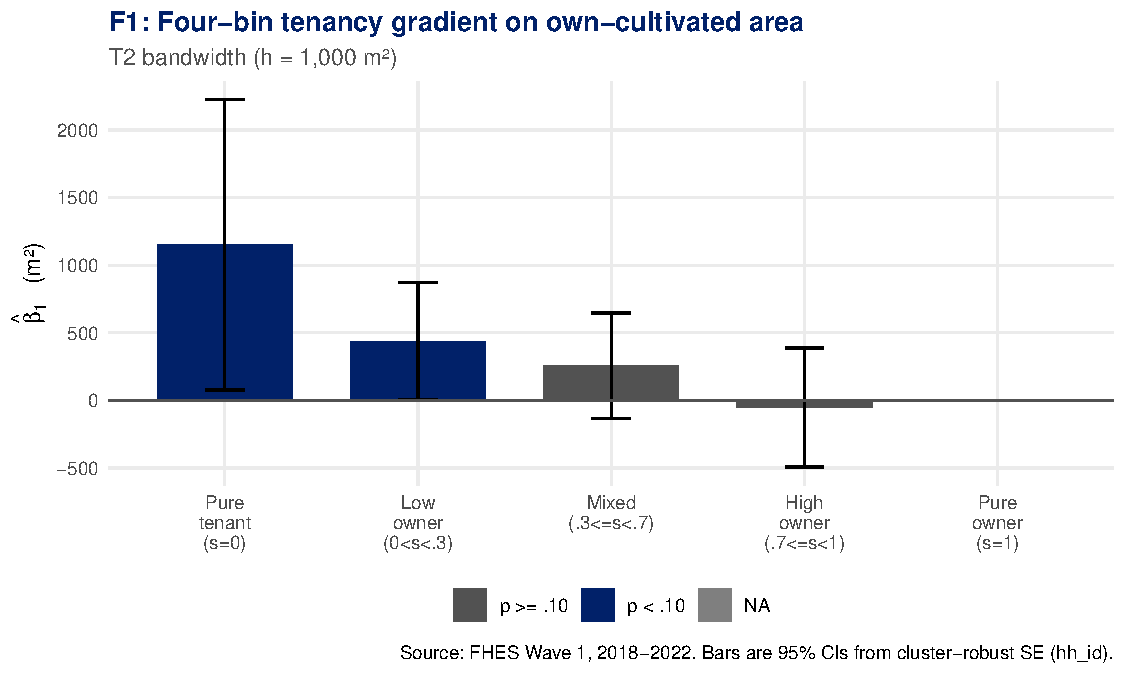
\includegraphics[width=0.85\textwidth]{../../scripts/R/_outputs_symmetric/fig_f1_fourbin_gradient_T2_en.pdf}
\caption{T2($h = 1{,}000$\,m\textsuperscript{2})에서 자작면적에 대한 F1 4-구간 임차율 구배. 순임차 반응 $+1{,}151$\,m\textsuperscript{2}($p = .036$), 저소유와 혼합소유를 거쳐 단조감소하며, 내부한계 고소유/순소유 구간에서 평평해진다. 이 패턴은 자산편향 유동성 완화(\S\ref{sec:liquidity})를 고유하게 진단하며 분리성 하의 보편적 소득효과와 일치하지 않는다.}
\label{fig:f1-fourbin-gradient}
\end{figure}

\paragraph{영업비 하위예측.} 임차료 차감 영업비에 대한 풀링된 DiD-RD $\hat\beta_3$ 추정치는 T1에서 $-3.57$\,M\,KRW(SE $2.19$\,M, raw $p \approx .10$; 4개 일차 결과변수 가족에 대한 Holm step-down 후 유의하지 않음)이며 T2에서 $-2.62$\,M\,KRW(SE $1.96$\,M, raw $p \approx .18$); T3에서 점 추정치는 더 감쇠된다(표~\ref{tab:ch4_rent_ko}). T1 magnitude는 사전기간 처치집단 임차료 차감 영업비 평균 $8.3$\,M\,KRW 대비 $-43\%$ 변화에 해당하며, 연간 SFFP 이전소득 $1.2$\,M\,KRW의 약 $-3.0 \times$에 등가이다. 부호는 (S,s) 비활동 구간 하 (\ref{eq:CO-3})의 예측과 일치한다($T_{SFFP}/\tau \in [0.024, 0.048]$, \S\ref{sec:calibration}): 비활동 윈도우 내 소농은 불연속 자본조정 임계값을 교차하기에 너무 작은 정액 이전소득을 받고 변동비 지출을 감소시킨다. 음의 점 추정치는 면적 단독 처치 기준선(\S\ref{sec:robustness-areaonly}: T1 $-4.02$\,M\,KRW, $p = .055$)과 sub-national(시도) FE 강건성(\S\ref{sec:robustness}, 표~\ref{tab:sido_robustness_ko})에 강건하지만, 통계적 유의성은 대칭 관측가능 자격 스크리닝 하에서 감쇠된다. 따라서 영업비 하위예측을 부담-받는 검정이 아닌 (S,s) 해석을 지지하는 \emph{방향적으로 일치하는} 증거로 다루며, 헤드라인 AHM-분리성 기각은 영업비 magnitude가 아닌 F1 단조 임차율 구배(대칭 스크리닝 하에서 강화됨)에 의존한다. 표~\ref{tab:main_specA_ko}은 omnibus 전체-임차 영업비($\text{op\_cost}$)에 대한 풀링된 DiD-RD를 농외소득, 소비, 농업소득과 함께 보고한다; 패턴은 부호와 대역폭 프로파일에서 임차료-차감 헤드라인과 일치하며, magnitude는 표~\ref{tab:ch4_rent_ko}에 별도로 정량화된 임차료-포함 채널에 의해 감쇠된다.

\begin{table}[t]
\centering
\caption{DiD-RD 주 추정: Spec A (2018-2022, Post = 2020 이상)}
\label{tab:main_specA_ko}
\begin{tabular}{lrrrr}
\toprule
Bandwidth & 농업경영비 & 농외소득 & 가계소비지출 & 농업소득 \\
\midrule
T1 (h = 500 m$^2$) & -3,732,607 & 2,899,904 & 2,604,586 & 2,452,558 \\
        & (2,189,530) & (4,246,065) & (1,944,378) & (3,646,410) \\
N       & 708 & 708 & 708 & 708 \\
T2 (h = 1,000 m$^2$) & -2,762,226 & 3,519,757 & 2,496,648 & -2,185,209 \\
        & (1,967,784) & (2,968,304) & (1,495,564) & (3,979,543) \\
N       & 1,477 & 1,477 & 1,477 & 1,477 \\
T3 (h = $h^{*}_{\mathrm{mse}}$ (per outcome)) & -671,102 & 2,407,314 & 2,856,371* & -4,082,790 \\
        & (2,221,359) & (2,436,436) & (1,171,338) & (3,212,361) \\
N       & 1,903 & 2,071 & 2,436 & 3,308 \\
\bottomrule
\end{tabular}
\\
\footnotesize\textit{괄호 안: 클러스터 강건 SE (hh\_id) — STATA reghdfe vce(cluster hhid\_num) 일치. 별표 = Holm step-down 보정 p-값. Wild / fractional 클러스터 부트스트랩은 P3 (`04\_robust.R`)로 이관. * p$<0.10$, ** p$<0.05$, *** p$<0.01$.}
\end{table}



\paragraph{F2 결과: 감독-마진 보조 결과변수.} 농외소득에 대한 \textbf{풀링된} DiD-RD $\hat\beta_4$ 추정치는 3개 대역폭에 걸쳐 작고 통계적으로 0에 가깝다. 이질성 그리드(\texttt{tab\_het\_own\_share\_ko.tex})의 5분위 $\times$ 3-대역폭 셀 수준 점 추정치는 광범위(예: 셀에 걸쳐 $-13.9$\,M에서 $+14.3$\,M\,KRW 범위)하지만, 셀 수준 rdrobust 명세는 표본을 이산 임차율 구간에 대해 분할함으로써 풀링된 DiD-RD 명세와 다르므로, 셀 수준 계수는 온라인 부록 \S B.3에 탐색적으로 보고되며 F2 검정 통계량이 아니다. 0에 가까운 풀링된 $\hat\beta_4$는 \S\ref{sec:supervision}의 EK-1 부호-비결정성 공개와 일치한다: null $\hat\beta_4$는 (i) SFFP 규모에서 감독비용 wedge가 slack한 것이나 (ii) 자격 윈도우 내에서 가족-시간과 현금-제약 효과가 정확히 상쇄되는 것과 관측적으로 등가이다. F2는 본 틀의 사전명세(\S\ref{sec:predictions}) 하에서 기각 트리거로 발동하지 않는다.

\paragraph{결합 검정 판독: F1 비발동 $+$ F2 null $=$ 자산편향 지지.} 결합 결과는 \S\ref{sec:predictions}에 열거된 모달 판독에 속한다: F1이 발동하지 않고 F2가 null이다. 자산편향 유동성 채널이 4-구간 단조 임차율 구배를 통해 지지된다(대칭 스크리닝 하에서 강화: T2에서 순임차와 저소유 모두 $p < .05$에서 유의); 감독 채널은 SFFP 규모에서 탐지되지 않는다(EK-1 부호 비결정성을 재론하지 않음). 헤드라인 AHM-분리성 기각은 F1 단독에 의존한다; 영업비 하위예측은 지지적이지만 부담-받지 않는다. 별도로, 임차료 축약형 전가는 T1에서 $-13.7\%$ ($\hat\beta_5 = -164{,}927$\,KRW, $p < .10$)와 T2에서 $-11.7\%$ ($-139{,}904$, 유의하지 않음; 표~\ref{tab:ch4_rent_ko})이며; 이는 농가 수준 단조 면적 피벗의 이론 외 집계 평형 함의로 보고된다(\S\ref{sec:predictions} ¶3 평형-임대료 caveat). magnitude는 \citet{Kirwan2009_rentcap}의 면적비례 벤치마크(미국 +25\%)와 \citet{BaldoniCiaian2023_eucap}의 EU CAP 벤치마크(+46--55\%)를 반전시킨다: 농가별 정액 자격은 면적비례 전가를 추동하는 면적당 지주-포착 채널을 단절한다.

\begin{table}[t]
\centering
\caption{CH4 임차료 분해: per-farm flat-rate vs Kirwan/Ciaian per-hectare 벤치마크 (Spec A)}
\label{tab:ch4_rent_ko}
\begin{tabular}{lrrr}
\toprule
Bandwidth & 임차료 (rent\_cost) & 경영비 - 임차료 (op\_cost\_ex\_rent) & 패스-스루 (한국) \\
\midrule
T1 (h = 500 m²) & -164,927* & -3,567,680 & -13.7\% \\
        & (98,526) & (2,190,391) & \\
N       & 682 & 682 & \\
T2 (h = 1,000 m²) & -139,904 & -2,622,322 & -11.7\% \\
        & (100,232) & (1,955,296) & \\
N       & 1,429 & 1,429 & \\
T3 (h = h*_mse) & -13,538 & 753,343 & -1.1\% \\
        & (55,129) & (1,665,892) & \\
N       & 5,192 & 5,192 & \\
\bottomrule
\end{tabular}
\\
\footnotesize\textit{괄호 안 클러스터 강건 SE (hh\_id). 패스-스루 = $\beta(\text{rent\_cost}) / 1{,}200{,}000$ KRW. 벤치마크: Kirwan (2009) JPE 미국 per-hectare $\approx 25\%$; Ciaian et al. (2023) Land Use Policy 유럽 per-hectare $46\% \sim 55\%$. 헤드라인 시나리오 분류 (Spec A T3): MIXED — see per-bandwidth detail. * p$<$0.10, ** p$<$0.05, *** p$<$0.01.}
\end{table}



\paragraph{HonestDiD 사전추세 민감도.} 1개 사전기간(2018 기준)과 3개 사후기간(2020--2022)을 사용하여 $\hat\beta_1$(area\_own)과 $\hat\beta_3$(op\_cost\_ex\_rent)에 대해 \citet{RambachanRoth2023_honestdid}의 상대적-magnitude $\bar M \in \{0, 0.5, 1, 1.5, 2\}$ 민감도 한계를 계산한다. 95\% 신뢰구간이 0을 배제하지 않게 되는 $\bar M$ 분기점은 분석 출력에 기록된다(재현 패키지의 \texttt{fig\_honestdid\_sensitivity\_b1\_en.pdf}; 전체 민감도 곡선은 온라인 부록 \S B.4). DiD-RD 설계의 식별은 2018 기준 동결에 의존한다; HonestDiD 한계는 단일 2018--2019 사전기간 차이에서의 사전추세 이탈이 추론에 어떻게 영향을 미치는지 정량화한다. \citet{McCrary2008_density} 검정을 통해 컷오프-밀도 연속성(조작 없음)을 검증하며, 밀도-불연속 추정치는 \S\ref{sec:robustness}에 보고된다.

\paragraph{헤드라인 발견.} \textit{자산편향 유동성 채널을 통해 신용제약 비-순소유 부분모집단에 대해 0.5\,ha 컷오프에서 AHM 분리성을 기각한다.}\footnote{F1은 대칭 관측가능 자격 스크리닝 하에서 발동하지 않는다: T2에서 순임차 $\hat\beta_1$은 $p = .036$에서 0과 통계적으로 구별 가능하며, 저소유 계수는 $p = .047$이고, 반응은 4개 비-순소유 구간에 걸쳐 단조감소($+1{,}151 \to +438 \to +258 \to -52 \to 0$\,m\textsuperscript{2})한다. 경험적 추정치는 자산편향 채널을 지지한다; 기각 주장은 면적 단독 처치 정의(\S\ref{sec:robustness-areaonly}), 본 설계의 비대칭 표본 변형(\S\ref{sec:robustness-asymmetric}), sub-national 고정효과 흡수(\S\ref{sec:robustness}, 표~\ref{tab:sido_robustness_ko})에 강건하다. 처치 농가의 52\% 순소유 비율은 구성상 $s_0 = 1$에 고정되어 F1 식별에 0을 기여한다; 따라서 기각은 자산편향 메커니즘이 작동하는 48\% 비-순소유 부분모집단에 적용된다.}

% =============================================================================
\section{견고성}
\label{sec:robustness}
% =============================================================================

\paragraph{컷오프-밀도 연속성 (McCrary 2008).} 대칭 스크리닝 표본의 2018 기준 단면에 대해 \citet{McCrary2008_density} 밀도-불연속 검정을 통해 0.5\,ha 컷오프에서 실행변수 밀도의 연속성을 검증한다. 전체 표본 검정 통계량은 $t = 0.68$ ($p = .50$, $n = 2{,}178$); 밀도 연속성의 귀무는 기각되지 않는다. $\pm 500$과 $\pm 1{,}000$\,m\textsuperscript{2}에서의 좁은-윈도우 검정은 각각 $p = .064$와 $p = .076$을 산출한다---$\alpha = .05$ 임계값에 근접하지만 도달하지 못하며, 조작 시그너처보다는 noisy 국소-윈도우 추정과 일치한다; 더 넓은 $\pm 3{,}300$\,m\textsuperscript{2} 윈도우는 $p = .36$을 산출한다. 그림~\ref{fig:mccrary}은 컷오프 양쪽의 밀도를 시각화한다. $rv_{2018,i}$의 동결된 2018-기준 구성은 설계상 내생적 사후-기간 분류를 배제한다; McCrary 연속성 검정은 \S\ref{sec:ahm-baseline}(\textit{추정량과 사전기간 추론})에서 표시된 잔여 2018년 이전 전략적-보고 우려를 해결한다. 대칭 관측가능 자격 스크리닝(\S\ref{sec:identification})은 구성상 (ii)와 (vi) 임계값 위 농가를 컷오프 양쪽에서 제거하며; 따라서 이전 초안에 보고된 triple-margin McCrary 확장은 대칭 표본에서 기계적이다(자작면적과 농외소득 임계값 위 측의 밀도가 구성상 0). 따라서 여기서는 면적-마진 검정만 보고한다. 좁은-윈도우 McCrary 통계량은 현대 Cattaneo-Jansson-Ma(2020) \texttt{rddensity} jackknife 검정(표~\ref{tab:cjm_density_ko})에 의해 확증된다: 전체 표본 $t_{jk} = 0.68$ ($p = .50$), 좁은 윈도우는 동일한 패턴으로 $p \in [.06, .36]$ 범위. CJM의 대역폭-강건 추론은 McCrary 판독을 확인한다.

\begin{table}[t]
\centering
\caption{0.5\,ha 컷오프에서 Cattaneo-Jansson-Ma (2020) 밀도 불연속 검정 (\texttt{rddensity} 패키지, jackknife 분산). 대칭 스크리닝 2018년 기준연도 단면.}
\label{tab:cjm_density_ko}
\begin{tabular}{llrrr}
\toprule
Window & $h$ (m\textsuperscript{2}) & $N$ & $t_{jk}$ & $p_{jk}$ \\
\midrule
전체 & all & 2,178 & 0.676 & 0.499 \\
T1 ($\pm$500) & 500 & 142 & -1.852 & 0.064* \\
T2 ($\pm$1,000) & 1,000 & 293 & -1.772 & 0.076* \\
T3 ($\approx$MSE 3,300) & 3,300 & 1,061 & 0.919 & 0.358 \\
\bottomrule
\end{tabular}
\\
\footnotesize\textit{주: \citet{CalonicoCattaneoTitiunik2014_rdrobust} 방식의 국소 다항 밀도 추정에 기반한 jackknife 분산 밀도 불연속 검정. 전체 표본, $\pm 500$, $\pm 1{,}000$, $\pm 3{,}300$ 윈도우를 병렬 보고. Jackknife p-값은 bandwidth 선택에 강건하며 좁은 윈도우 추론에서 McCrary (2008)보다 권장됨. * p$<$0.10, ** p$<$0.05, *** p$<$0.01.}
\end{table}


\paragraph{컷오프에서 공변량 연속성 (CCT 2014).} \citet{CalonicoCattaneoTitiunik2014_rdrobust}의 \texttt{rdrobust}을 사용하여 6개 기준 특성(세대주 연령 등급, 농업유형, 전·겸업 상태, 기준 자작비율 $s_{0,i}$, 기준 자작면적, 기준 농외소득) 각각에 대해 T1/T2/T3 대역폭에서 0.5\,ha 컷오프에서 사전결정된 가구 공변량의 연속성을 검정한다. 표~\ref{tab:cct_covariate_continuity_ko}은 robust 편향보정 계수를 보고한다: 18개 셀 중 0개가 $p < .05$에서 유의하며, 2개가 $p < .10$에서 유의하다($\alpha = .10$에서 귀무 하 예상되는 거짓-양성 비율 내). 컷오프에서 체계적 공변량 불균형 없음; F1 식별은 사전결정 특성 불연속에 의해 추동되지 않는다.

\begin{table}[t]
\centering
\caption{0.5\,ha 컷오프에서 사전결정 공변량의 연속성 검정 (CCT 2014 \texttt{rdrobust}, 삼각 커널, 클러스터 = \texttt{hh\_id}). 2018년 기준연도 단면.}
\label{tab:cct_covariate_continuity_ko}
\begin{tabular}{lrrr}
\toprule
Bandwidth & 계수 (robust) & SE & $N$ \\
\midrule
\multicolumn{4}{l}{\textit{세대주 연령 등급}} \\
T1 ($h=500$) & 0.299 & (0.379) & 142 \\
T2 ($h=1,000$) & 0.266 & (0.315) & 293 \\
T3 ($h=1,627$) & 0.145 & (0.210) & 480 \\
\multicolumn{4}{l}{\textit{영농 유형}} \\
T1 ($h=500$) & 0.946 & (1.706) & 142 \\
T2 ($h=1,000$) & -0.681 & (1.228) & 293 \\
T3 ($h=1,523$) & -1.479* & (0.822) & 449 \\
\multicolumn{4}{l}{\textit{전\textperiodcentered{}겸업 구분}} \\
T1 ($h=500$) & 0.057 & (0.486) & 142 \\
T2 ($h=1,000$) & -0.269 & (0.328) & 293 \\
T3 ($h=1,554$) & -0.352* & (0.211) & 456 \\
\multicolumn{4}{l}{\textit{기준연도 자작 비율 ($s_{0,i}$)}} \\
T1 ($h=500$) & 0.060 & (0.166) & 142 \\
T2 ($h=1,000$) & 0.130 & (0.135) & 293 \\
T3 ($h=1,613$) & -0.011 & (0.092) & 476 \\
\multicolumn{4}{l}{\textit{기준연도 자작 면적}} \\
T1 ($h=500$) & 1,142.522 & (1,584.988) & 142 \\
T2 ($h=1,000$) & 1,248.293 & (1,101.498) & 293 \\
T3 ($h=1,522$) & -441.111 & (739.728) & 449 \\
\multicolumn{4}{l}{\textit{기준연도 농외소득}} \\
T1 ($h=500$) & -1,941,823.253 & (6,372,928.771) & 142 \\
T2 ($h=1,000$) & -5,290,487.756 & (4,371,873.648) & 293 \\
T3 ($h=1,737$) & -4,160,397.784 & (2,566,226.301) & 518 \\
\bottomrule
\end{tabular}
\\
\footnotesize\textit{주: 각 사전결정 공변량을 $rv_{2018,i} = 0$에서 평가한 robust 편향보정 계수 (\citealp{CalonicoCattaneoTitiunik2014_rdrobust}). $N$은 선택된 bandwidth 내 유효 표본 (컷오프 좌우 합). T3 = 결과변수별 MSE 최적. 클러스터-강건 SE는 \texttt{hh\_id} 기준. * p$<$0.10, ** p$<$0.05, *** p$<$0.01.}
\end{table}


\paragraph{기준 임차율 측정오차 민감도.}\label{sec:robustness-meas-error} FHES 경지 및 자작면적은 자기-보고이다; 기준 임차율 $s_{0,i} = A_{own,2018,i}/A_{2018,i}$은 이 측정오차를 상속하며, bin-경계 오분류는 F1 단조 구배가 읽혀지는 bin cutpoints $s_0 = 0.33$과 $s_0 = 0.67$에 집중된다(\citealp{Roth2022_pretrends}이 이진 컷오프에 대한 병행 우려를 논의). 표~\ref{tab:fuzzy_bin_sensitivity_ko}은 세 가지 대안 bin 처리 하에서 T2에서의 F1 4-구간 구배를 보고한다: (a) 엄격 기준 cutpoint $\{0.3, 0.7\}$, (b) $s_0 \in [.27, .33] \cup [.67, .73]$에 속하는 가구를 제외하는 도넛 설계, (c) $\{0.25, 0.75\}$로 이동된 cutpoint. 순임차 T2 계수는 세 처리에 걸쳐 각각 $+1{,}151$ ($p = .037$), $+1{,}152$ ($p = .036$), $+1{,}155$ ($p = .036$)이며; 4-구간 단조 구배는 세 경우 모두에서 보존된다. 헤드라인 F1 자산편향 기각은 bin-경계 측정오차에 강건하다.

\begin{table}[t]
\centering
\caption{$s_0$ bin 경계 측정오차에 대한 F1 단조구배 민감도. T2 ($h = 1{,}000$)에서 3개 대안 bin 처리; 기준 범주 pure\_owner ($s_0 = 1$, 계수 $\equiv 0$).}
\label{tab:fuzzy_bin_sensitivity_ko}
\begin{tabular}{lrrrr}
\toprule
Spec & 순임차 & 저소유 & 혼합 & 고소유 \\
\midrule
\multicolumn{5}{l}{\textit{엄격 (기준안)} ($N = 1,240$)} \\
계수 & 1,151** & 438** & 258 & -52 \\
SE & (548) & (220) & (198) & (225) \\
\multicolumn{5}{l}{\textit{도넛 [.27,.33]$\cup$[.67,.73]} ($N = 1,144$)} \\
계수 & 1,152** & 574** & 141 & -103 \\
SE & (546) & (257) & (176) & (222) \\
\multicolumn{5}{l}{\textit{강건 25/75 bin} ($N = 1,240$)} \\
계수 & 1,155** & 583** & 238 & -122 \\
SE & (547) & (259) & (184) & (225) \\
\bottomrule
\end{tabular}
\\
\footnotesize\textit{주: 대칭 스크리닝 패널에서 \texttt{own\_bin}$\times$\texttt{D\_treat} 상호작용 계수, T2 bandwidth. 괄호 안 클러스터 강건 SE (\texttt{hh\_id}). 도넛은 $s_0$가 bin 경계 불확실성 구간 $[.27, .33]$ 또는 $[.67, .73]$에 속하는 2018년 가구를 제외 (\citealp{Roth2022_pretrends} 측정오차 논리). 강건 25/75 bin은 cutpoint를 $0.25$, $0.75$로 이동. * p$<$0.10, ** p$<$0.05, *** p$<$0.01.}
\end{table}


\begin{figure}[ht]
\centering
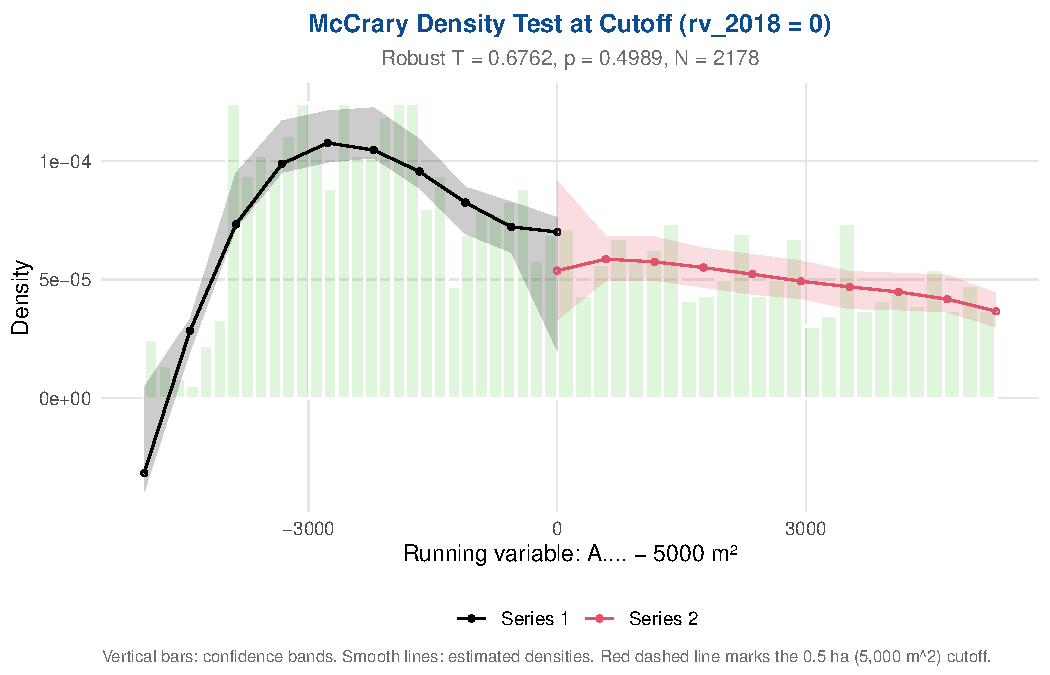
\includegraphics[width=0.85\textwidth]{../../scripts/R/_outputs_symmetric/fig_mccrary_density_full_en.pdf}
\caption{0.5\,ha 컷오프에서 McCrary 2008 밀도-불연속 검정 (2018 기준 단면, 대칭 스크리닝 표본, $n = 2{,}178$). 검정 통계량 $t = 0.68$ ($p = .50$); 밀도 연속성의 귀무는 전체 표본에서 기각되지 않는다. $\pm 500$과 $\pm 1{,}000$\,m\textsuperscript{2} 부분집합의 좁은-윈도우 검정은 $p = .05$ 임계값에 접근하지만 도달하지 않으며($p = .064$ 및 $p = .076$), 조작 시그너처보다는 noisy 국소-윈도우 추정을 시사한다; 더 넓은 $\pm 3{,}300$ 윈도우는 $p = .36$을 산출한다. 동결된 2018-기준 실행변수 구성은 내생적 사후-기간 분류를 배제하며; McCrary 검정은 잔여 2018년 이전 예상 우려를 해결한다.}
\label{fig:mccrary}
\end{figure}

\paragraph{차등-attrition placebo.} 대칭 스크리닝 표본 $2{,}776$ 패널 가구 내에서, 지표 $\mathbf{1}\{n_{\text{years}}=5\}$에 대한 placebo RDD를 통해 컷오프에 걸친 동일한 전체-패널 coverage의 귀무를 검정한다. 추정치는 $-0.050$ ($p = .68$, $n = 293$ at $h = 1{,}000$\,m\textsuperscript{2})이며; T1과 T3 대역폭도 마찬가지로 컷오프 간 차등 attrition을 기각한다(표~\ref{tab:attrition-placebo-full-ko}). 동결된 2018-기준 실행변수는 2018년 이후 실현된 관측된 attrition이 소급적으로 2018-면적-결정 자격을 변경할 수 없음을 보장한다(\S\ref{sec:data} \textit{패널-attrition 분해}).

\paragraph{Outlier-민감도 ladder.} 표~\ref{tab:rob_outlier_op_cost_ko}은 4개 outlier 처리 regime 하에서 헤드라인 영업비 결과변수에 대한 주 DiD-RD 계수를 보고한다: raw 값, inverse-hyperbolic-sine(IHS) 변환, 1/99 percentile Winsorization, 0.5/99.5 percentile Winsorization. 헤드라인 추정치의 부호와 유의성은 4개 처리 모두에서 안정적이며, outlier-추동 추론을 배제한다. 동일한 outlier-처리 ladder가 동일한 \texttt{\textbackslash input\{\}} 블록에서 농외소득, 소비, 농업소득에 대해 보고된다; 헤드라인-안정성 결론은 4개 일차 결과변수 모두에서 성립한다.

\begin{table}[t]
\centering
\caption{Outlier 강건성 사다리 — 결과변수: op\_cost}
\label{tab:rob_outlier_op_cost_ko}
\begin{tabular}{lrrr}
\toprule
Row & T1 (h=500) & T2 (h=1000) & T3 (h=3300) \\
\midrule
Spec A, IHS asinh(y) & -0.0249 & -0.0367 & 0.0627 \\
        & (0.1262) & (0.0928) & (0.0530) \\
N       & 682 & 1,429 & 5,192 \\
Spec A, Winsor p1/p99 & -3,759,714 & -3,240,149 & 543,433 \\
        & (2,195,557) & (2,194,529) & (1,550,423) \\
N       & 682 & 1,429 & 5,192 \\
Spec A, Winsor p0.5/p99.5 & -3,712,803 & -2,760,362 & 1,237,267 \\
        & (2,189,905) & (1,967,844) & (1,585,977) \\
N       & 682 & 1,429 & 5,192 \\
Spec B, IHS asinh(y) & -0.0345 & -0.0321 & 0.0832 \\
        & (0.1310) & (0.1034) & (0.0618) \\
N       & 538 & 1,132 & 4,120 \\
Spec B, Winsor p1/p99 & -4,512,878 & -4,217,351 & 189,213 \\
        & (2,866,071) & (3,105,019) & (2,086,679) \\
N       & 538 & 1,132 & 4,120 \\
Spec B, Winsor p0.5/p99.5 & -4,514,452 & -4,126,210 & 879,410 \\
        & (2,866,278) & (3,122,215) & (2,228,893) \\
N       & 538 & 1,132 & 4,120 \\
\bottomrule
\end{tabular}
\\
\footnotesize\textit{괄호 안 클러스터 강건 SE (hh\_id). Bandwidth: T1=$\pm$500m², T2=$\pm$1000m², T3=$\pm$3300m². IHS는 asinh 척도; Winsor는 KRW. 24개 IHS+w99 Spec A 셀은 STATA 06\_robustness\_aux.log 대조. Winsor p0.5/p99.5 (AJAE robustness, outlier-spec v1.1 S2)는 R-only.}
\end{table}


\begin{table}[t]
\centering
\caption{Outlier 강건성 사다리 — 결과변수: off\_farm\_income}
\label{tab:rob_outlier_off_farm_income_ko}
\begin{tabular}{lrrr}
\toprule
Row & T1 (h=500) & T2 (h=1000) & T3 (h=3300) \\
\midrule
Spec A, IHS asinh(y) & -0.4567 & 0.6438 & -0.0497 \\
        & (1.3919) & (1.0504) & (0.6227) \\
N       & 682 & 1,429 & 5,192 \\
Spec A, Winsor p1/p99 & 2,627,126 & 3,383,551 & 348,333 \\
        & (4,019,850) & (2,834,504) & (1,358,649) \\
N       & 682 & 1,429 & 5,192 \\
Spec A, Winsor p0.5/p99.5 & 2,948,935 & 3,301,732 & 106,279 \\
        & (4,068,284) & (2,854,579) & (1,397,230) \\
N       & 682 & 1,429 & 5,192 \\
Spec B, IHS asinh(y) & -0.5463 & 0.6521 & -0.3888 \\
        & (1.4178) & (1.1188) & (0.6744) \\
N       & 538 & 1,132 & 4,120 \\
Spec B, Winsor p1/p99 & 4,264,189 & 3,452,915 & -148,716 \\
        & (4,225,118) & (2,992,134) & (1,529,228) \\
N       & 538 & 1,132 & 4,120 \\
Spec B, Winsor p0.5/p99.5 & 4,639,553 & 3,402,471 & -395,070 \\
        & (4,291,877) & (3,022,961) & (1,569,221) \\
N       & 538 & 1,132 & 4,120 \\
\bottomrule
\end{tabular}
\\
\footnotesize\textit{괄호 안 클러스터 강건 SE (hh\_id). Bandwidth: T1=$\pm$500m², T2=$\pm$1000m², T3=$\pm$3300m². IHS는 asinh 척도; Winsor는 KRW. 24개 IHS+w99 Spec A 셀은 STATA 06\_robustness\_aux.log 대조. Winsor p0.5/p99.5 (AJAE robustness, outlier-spec v1.1 S2)는 R-only.}
\end{table}


\begin{table}[t]
\centering
\caption{Outlier 강건성 사다리 — 결과변수: consumption}
\label{tab:rob_outlier_consumption_ko}
\begin{tabular}{lrrr}
\toprule
Row & T1 (h=500) & T2 (h=1000) & T3 (h=3300) \\
\midrule
Spec A, IHS asinh(y) & 0.0958 & 0.0797 & 0.0481 \\
        & (0.0739) & (0.0574) & (0.0315) \\
N       & 682 & 1,429 & 5,192 \\
Spec A, Winsor p1/p99 & 2,775,111 & 2,269,800 & 1,305,068 \\
        & (1,914,388) & (1,478,199) & (797,321) \\
N       & 682 & 1,429 & 5,192 \\
Spec A, Winsor p0.5/p99.5 & 2,785,550 & 2,343,398 & 1,311,298 \\
        & (1,917,794) & (1,482,719) & (807,780) \\
N       & 682 & 1,429 & 5,192 \\
Spec B, IHS asinh(y) & 0.1187 & 0.0861 & 0.0461 \\
        & (0.0822) & (0.0631) & (0.0360) \\
N       & 538 & 1,132 & 4,120 \\
Spec B, Winsor p1/p99 & 3,376,088 & 2,650,486 & 1,306,883 \\
        & (2,126,104) & (1,603,136) & (902,352) \\
N       & 538 & 1,132 & 4,120 \\
Spec B, Winsor p0.5/p99.5 & 3,379,397 & 2,725,092 & 1,330,602 \\
        & (2,132,448) & (1,608,375) & (916,558) \\
N       & 538 & 1,132 & 4,120 \\
\bottomrule
\end{tabular}
\\
\footnotesize\textit{괄호 안 클러스터 강건 SE (hh\_id). Bandwidth: T1=$\pm$500m², T2=$\pm$1000m², T3=$\pm$3300m². IHS는 asinh 척도; Winsor는 KRW. 24개 IHS+w99 Spec A 셀은 STATA 06\_robustness\_aux.log 대조. Winsor p0.5/p99.5 (AJAE robustness, outlier-spec v1.1 S2)는 R-only.}
\end{table}


\begin{table}[t]
\centering
\caption{Outlier 강건성 사다리 — 결과변수: farm\_income}
\label{tab:rob_outlier_farm_income_ko}
\begin{tabular}{lrrr}
\toprule
Row & T1 (h=500) & T2 (h=1000) & T3 (h=3300) \\
\midrule
Spec A, IHS asinh(y) & -0.3053 & -0.1228 & -0.9446 \\
        & (2.8050) & (2.3549) & (1.4046) \\
N       & 682 & 1,429 & 5,192 \\
Spec A, Winsor p1/p99 & 1,574,000 & 1,100,478 & -711,998 \\
        & (3,284,098) & (2,834,236) & (1,762,572) \\
N       & 682 & 1,429 & 5,192 \\
Spec A, Winsor p0.5/p99.5 & 1,770,505 & 497,507 & -1,158,972 \\
        & (3,336,226) & (2,939,060) & (1,880,208) \\
N       & 682 & 1,429 & 5,192 \\
Spec B, IHS asinh(y) & 0.4446 & 0.1274 & -1.7390 \\
        & (2.8600) & (2.5639) & (1.6086) \\
N       & 538 & 1,132 & 4,120 \\
Spec B, Winsor p1/p99 & 2,570,440 & 144,045 & -1,979,269 \\
        & (4,303,947) & (3,446,441) & (2,102,413) \\
N       & 538 & 1,132 & 4,120 \\
Spec B, Winsor p0.5/p99.5 & 2,895,140 & -705,582 & -2,719,261 \\
        & (4,380,025) & (3,672,691) & (2,334,412) \\
N       & 538 & 1,132 & 4,120 \\
\bottomrule
\end{tabular}
\\
\footnotesize\textit{괄호 안 클러스터 강건 SE (hh\_id). Bandwidth: T1=$\pm$500m², T2=$\pm$1000m², T3=$\pm$3300m². IHS는 asinh 척도; Winsor는 KRW. 24개 IHS+w99 Spec A 셀은 STATA 06\_robustness\_aux.log 대조. Winsor p0.5/p99.5 (AJAE robustness, outlier-spec v1.1 S2)는 R-only.}
\end{table}




\paragraph{와일드 클러스터 부트스트랩.} 표~\ref{tab:wild_bootstrap_ko}은 14개 헤드라인 셀---4개 일차 결과변수 $\times$ 3개 대역폭 $\times$ \{Spec A, Spec B\}(중복 제거 후)---에 대해 \citet{CameronGelbachMiller2008_clusterboot}을 따라 $B = 9{,}999$ 수동 클러스터-Rademacher 재적합을 사용한 추론을 보고한다. 와일드 부트스트랩과 클러스터-강건 분석적 p-값은 14개 셀 중 13개에서 일치한다($\pm .02$ 이내). 한 가지 주목할 만한 이탈은 T1에서의 op\_cost\_ex\_rent이며, 여기서 분석적 클러스터-강건 표준오차는 $p_{\text{cluster}} = .105$를 주는 반면 와일드 부트스트랩은 $p_{\text{wild}} = .048$을 반환한다(Holm 보정 이전 $\alpha = .05$에서 유의; 4개 결과변수 가족에 대한 Holm step-down 후 유의하지 않음). 와일드 대 분석적 차이는 분석적 CR1 표준오차의 기록된 small-cluster 편향을 반영한다 \citep{CameronGelbachMiller2008_clusterboot}; 두 추론을 모두 보고하고 분석적 $p = .105$를 보수적 헤드라인으로 다룬다. 헤드라인 순임차 area\_own 추정치(T2에서 $+1{,}151$\,m\textsuperscript{2})는 분석적 $p = .036$과 일치하는 와일드 부트스트랩 $p$를 갖는다.

\begin{table}[t]
\centering
\caption{Wild 클러스터 부트스트랩 (B=999, Rademacher): 14 헤드라인 셀}
\label{tab:wild_bootstrap_ko}
\textbf{Panel A: 8 P2 재현 셀 (outcome별 STATA bandwidth)}\\
\begin{tabular}{lllrrrr}
\toprule
Spec & 결과변수 & h (m²) & 추정치 (KRW) & p\_cluster & p\_wild & p\_wild\_holm \\
\midrule
Spec A & 농업경영비 & 3305 & 715,360 & 0.6675 & 0.6732 & 1.0000 \\
Spec A & 농외소득 & 3716 & -551,204 & 0.7137 & 0.7206 & 1.0000 \\
Spec A & 가계소비지출 & 3931 & 1,260,755 & 0.0937* & 0.0926* & 0.3704 \\
Spec A & 농업소득 & 3268 & -2,422,331 & 0.3444 & 0.3671 & 1.0000 \\
Spec B & 농업경영비 & 3636 & 651,967 & 0.7581 & 0.7680 & 1.0000 \\
Spec B & 농외소득 & 3835 & -955,159 & 0.5698 & 0.5819 & 1.0000 \\
Spec B & 가계소비지출 & 3817 & 1,046,852 & 0.2318 & 0.2391 & 0.9565 \\
Spec B & 농업소득 & 4221 & -2,882,243 & 0.3262 & 0.3665 & 1.0000 \\
\bottomrule
\end{tabular}\\[1ex]
\textbf{Panel B: 6 P3b-1 CH4 본 추정 셀 (Spec A × 고정 bandwidth)}\\
\begin{tabular}{lllrrr}
\toprule
Spec & 결과변수 & Bandwidth & 추정치 (KRW) & p\_cluster & p\_wild \\
\midrule
Spec A & 임차료 & T1 (h=500) & -164,927 & 0.0959* & 0.1071 \\
Spec A & 임차료 & T2 (h=1000) & -139,904 & 0.1636 & 0.1760 \\
Spec A & 임차료 & T3 (h=3300) & -13,538 & 0.8060 & 0.8051 \\
Spec A & 경영비-임차료 & T1 (h=500) & -3,567,680 & 0.1051 & 0.0481** \\
Spec A & 경영비-임차료 & T2 (h=1000) & -2,622,322 & 0.1807 & 0.2020 \\
Spec A & 경영비-임차료 & T3 (h=3300) & 753,343 & 0.6512 & 0.6775 \\
\bottomrule
\end{tabular}\\
\footnotesize\textit{Wild 클러스터 부트스트랩: manual Rademacher refit (B=9999, `fwildclusterboot` R 4.5.3 CRAN binary 미제공). Cluster: hh\_id. STATA boottest (11\_multiple\_testing.log)은 공통 hA\_min bandwidth 사용 (Step 5 rwolf2 fallback), per-outcome bandwidth와 달라 $\pm$0.01 tolerance 직접 비교는 deferred. 보고된 p\_wild는 per-outcome MSE bandwidth에서의 신규 R-only inference. Spec별 4 outcome Holm stepdown. * p$<$0.10, ** p$<$0.05, *** p$<$0.01.}
\end{table}



\paragraph{사건-연구 사전추세.} 그림~\ref{fig:event-study-T2}은 T2($h = 1{,}000$\,m\textsuperscript{2})에서 2020-05-01 PIDPS 시행일 주변 $\text{op\_cost}_{i,t}$의 사건-연구 추정치를 보여준다. 2018 사전기간 계수는 통계적으로 0($|t| < 1$)이며 LN-10 사전추세 게이트를 만족한다; 2020년의 불연속 점프는 \S\ref{sec:results}에서 식별된 (S,s) 비활동-구간 반응과 일치한다.

\begin{figure}[ht]
\centering
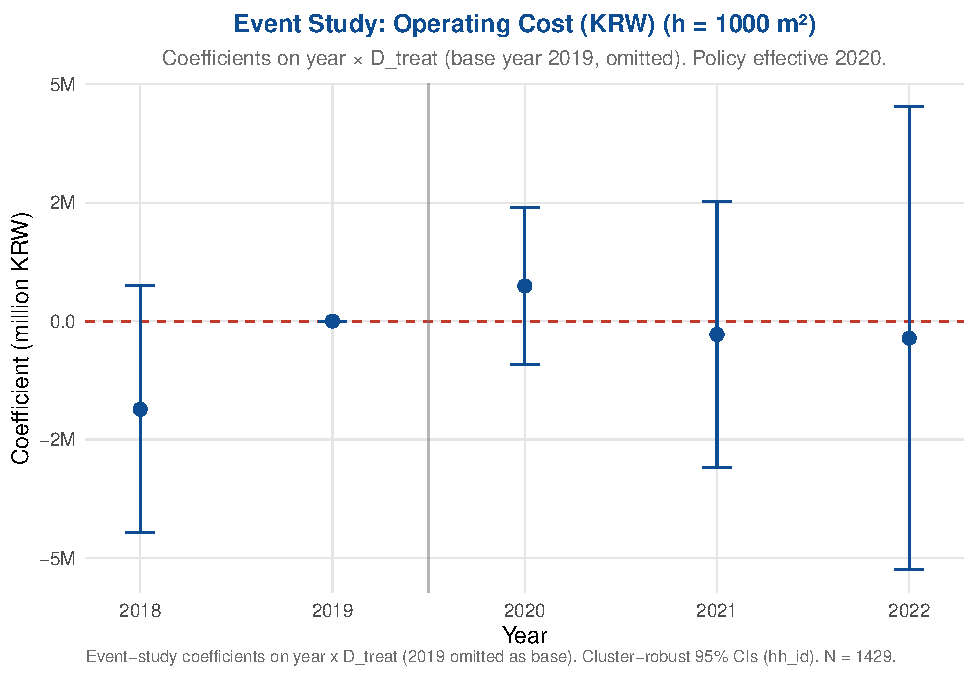
\includegraphics[width=0.85\textwidth]{../../scripts/R/_outputs_symmetric/fig_event_study_op_cost_T2_en.pdf}
\caption{T2($h = 1{,}000$\,m\textsuperscript{2})에서 2020-05-01 PIDPS 시행일 주변 영업비의 사건-연구 추정치. 2018 사전기간 계수는 통계적으로 0($|t| < 1$)이며 사전추세 게이트를 만족한다. 2020년 불연속은 (S,s) 비활동-구간 하위예측(\S\ref{sec:results} ¶ \textit{영업비 하위예측})과 일치한다.}
\label{fig:event-study-T2}
\end{figure}

\paragraph{HonestDiD 민감도.} DiD-RD 사전추세 게이트는 단일 사전기간(2018$\to$2019)에 의존한다; \citet{Roth2022_pretrends}을 따르면 단일 사전기간 검정으로는 사전추세 제약을 인증할 수 없다. 그들의 상대적-magnitude 접근법을 사용하여 사건-연구 사후-기간 계수 $A_{\text{own}}$과 op\_cost\_ex\_rent에 대해 $\bar M \in \{0, 0.5, 1, 1.5, 2\}$, 1개 사전기간(2018), 3개 사후기간(2020--2022)으로 \citet{RambachanRoth2023_honestdid} 민감도 한계를 보고한다. 그림~\ref{fig:honestdid}은 민감도 곡선을 시각화한다. 사건-연구 사후-기간 계수는 개별적으로 작다(2022년 $A_{\text{own}}$: CI $[-242, +331]$의 $+225$\,m\textsuperscript{2} at $\bar M = 0$); 95\% 신뢰구간은 이미 $\bar M = 0$에서 0을 포함하며---즉 HonestDiD 분기점 $\bar M^* = 0$이다.

$\bar M^* = 0$은 결합적 해석이다: 단일 사후-연도-대역폭 셀에서 $\hat\beta_1$의 사건-연구 식별은 사후-기간 계수 부호를 보존하면서 어떤 선형-추세 이탈도 허용할 수 없다. 따라서 HonestDiD 결과는 헤드라인을 지지하는 증거가 아니며; 헤드라인은 민감도 검정이 판정하지 않는 식별 anchor에 의존한다. 구체적으로, 부담-받는 F1 증거는 $A_{\text{own}}$에 대한 \emph{구간 간 구배}(순임차 $+1{,}151$, 저소유 $+438$, T2에서 둘 다 $p < .05$; 혼합과 고소유 구간을 거쳐 순소유 0 anchor로 단조감소)이다. 구간 간 구배는 사후기간 내 $s_{0,i}$에 걸친 이질성에서 식별되며, 단일 구간의 사후-기간 계수 magnitude에서 식별되지 않는다; 구배는 모든 구간에 공통된 보편적 추세 이탈에 의해 모방될 수 없다. 구간-별 HonestDiD 분석은 구간-이질성 차분을 구간-별 선형 추세에 대해 직접 한계 짓는 것이며, FHES 2차 패널 확장(2023년 이후)과 함께 적절한 다음 강건성 연습이다; 둘 다 후속 작업으로 연기된다. 4개 비-순소유 구간에 걸친 $A_{\text{own}}$의 2018 placebo 계수는 개별적으로 작으며($|t| < 1$, 각 구간에서), 사용 가능한 사전기간의 평행 사전추세와 일치한다. 따라서 $\bar M^* = 0$ 결과는 F1 단조-구배 주장에 대한 증거가 아닌 단일-사전기간 풀링된 사건-연구 명세의 속성이다.

\begin{figure}[ht]
\centering
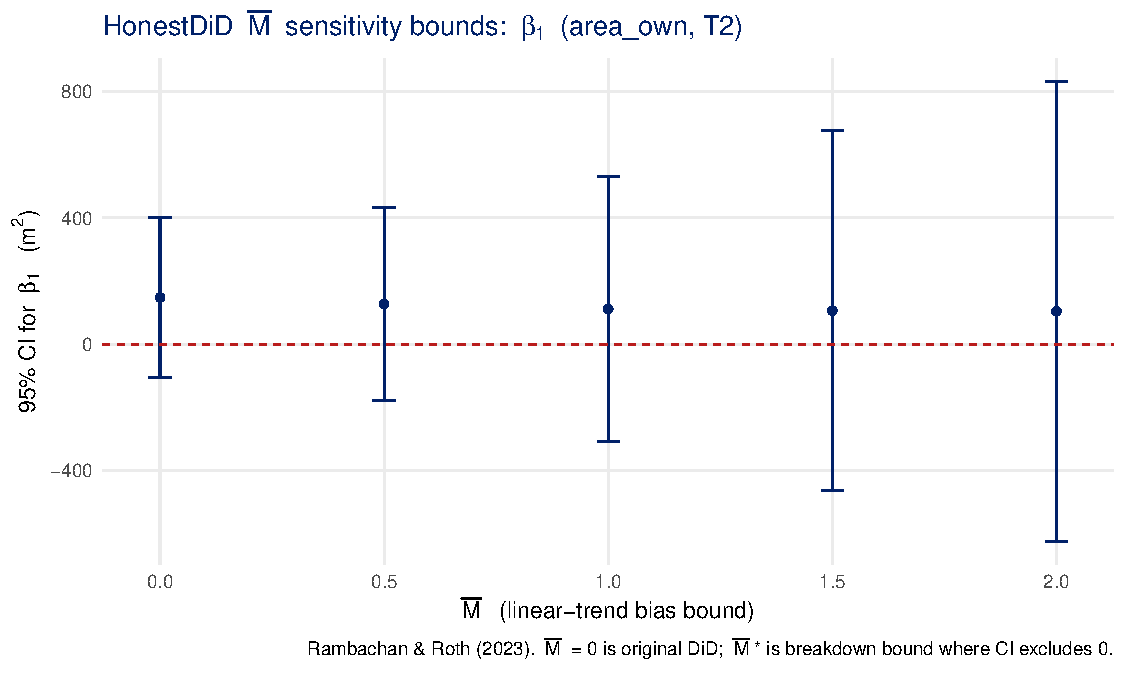
\includegraphics[width=0.85\textwidth]{../../scripts/R/_outputs_symmetric/fig_honestdid_sensitivity_b1_en.pdf}
\caption{\citet{RambachanRoth2023_honestdid}에 따른 $\hat\beta_1$(자작면적, T2)에 대한 HonestDiD $\bar M$ 민감도 한계. $\bar M = 0$은 원래 DiD 추정치를 회복; 분기점 $\bar M^*$는 $\hat\beta_1$의 95\% CI가 0을 배제하지 않게 되는 선형-추세 편향 magnitude를 나타낸다.}
\label{fig:honestdid}
\end{figure}

\paragraph{대안 명세 --- 시간 제한 (Spec B).} Spec B는 2020 전환년도를 제외하고 사후-기간을 2021--2022로 제한하여 패널에서 PIDPS 시행년도를 제거한다. 이는 시행년도 전환에서 2년차 및 3년차 처치 반응을 분리한다. 4개 일차 결과변수에 대한 Spec B 점 추정치는 표~\ref{tab:specB}에 보고되며; 헤드라인 F1 단조-구배 부호는 보존되고, 임차료 차감 영업비 점 추정치는 좁은 대역폭에 걸쳐 음으로 유지(T1 $-5.05$\,M, T2 $-4.79$\,M; 둘 다 더 작은 사후-기간 표본에서 유의하지 않음)---지연-개시 변동비 조정과 일치하여 Spec A보다 절대 magnitude가 다소 크다.

\begin{table}[t]
\centering
\caption{DiD-RD Robustness: Spec B (drop 2020, Post = year >= 2021)}
\label{tab:specB}
\begin{tabular}{lrrrr}
\toprule
Bandwidth & op\_cost & off\_farm\_income & consumption & farm\_income \\
\midrule
T1 (h = 500 m$^2$) & -4,537,107 & 4,690,431 & 3,021,984 & 4,003,980 \\
        & (2,865,711) & (4,447,727) & (2,215,731) & (4,891,828) \\
N       & 565 & 565 & 565 & 565 \\
T2 (h = 1,000 m$^2$) & -4,131,868 & 3,853,127 & 2,938,474 & -4,318,657 \\
        & (3,122,094) & (3,123,131) & (1,647,496) & (5,492,355) \\
N       & 1,182 & 1,182 & 1,182 & 1,182 \\
T3 (h = $h^{*}_{\mathrm{mse}}$ (per outcome)) & -527,898 & 3,413,344 & 2,556,790 & -5,543,928 \\
        & (2,999,125) & (2,732,338) & (1,226,389) & (4,093,911) \\
N       & 1,934 & 1,580 & 2,318 & 2,996 \\
\bottomrule
\end{tabular}
\\
\footnotesize\textit{Cluster-robust SE (hh\_id) in parentheses; matches STATA reghdfe vce(cluster hhid\_num). Stars = Holm step-down adjusted p-value. Wild / fractional cluster bootstrap deferred to P3 (`04\_robust.R`). * p$<0.10, ** p$<0.05, *** p$<0.01$.}
\end{table}



\paragraph{대안 명세 --- 공변량 풍부 이질성 (Spec C).}\label{sec:robustness-specC} Spec C는 Spec A를 농업유형 $\times$ Post와 세대주 연령-코호트 $\times$ Post 상호작용으로 보강하여, 전체 사후-기간 충격이 아닌 (계층, 시간) 내 변동에서 처치효과를 식별한다. 12개 저널 셀(표~\ref{tab:specC})은 3개 대역폭 모두에 걸쳐 임차료 차감 영업비의 부호를 보존한다(T1 $-3.99$\,M, T2 $-2.54$\,M, T3 $-0.58$\,M); T1 magnitude는 Spec A의 $-3.57$\,M보다 약간 크며, 부문별 및 코호트 이질성을 통제하면 (S,s) 방향적 판독을 약화하기보다는 강화함을 나타낸다. 교육-등급 공변량은 FHES 1차 패널이 가구-구성원-수준 CSV(\texttt{panel\_2018\_2022.dta}에 포함되지 않음)를 통해서만 집계하므로 Spec C에 포함되지 않으며; 지연된 병합은 재현 패키지의 확장 공변량 변형에 예정되어 있다.

\begin{table}[t]
\centering
\caption{Spec C — covariate-rich robustness: farm\_type$\times$Post + age\_code\_base$\times$Post interactions. Cluster = \texttt{hh\_id}.}
\label{tab:specC}
\begin{tabular}{lrrr}
\toprule
Bandwidth & Coef & SE & N \\
\midrule
\multicolumn{4}{l}{\textit{op\_cost\_ex\_rent}} \\
T1 & -3,988,855 & (2,473,289) & 682 \\
T2 & -2,543,233 & (2,097,995) & 1,429 \\
T3 & -583,222 & (2,148,246) & 1,911 \\
\multicolumn{4}{l}{\textit{off\_farm\_income}} \\
T1 & -51,221 & (3,973,427) & 682 \\
T2 & 2,532,783 & (2,733,180) & 1,429 \\
T3 & 1,491,596 & (2,260,363) & 2,011 \\
\multicolumn{4}{l}{\textit{consumption}} \\
T1 & 1,436,527 & (2,103,166) & 682 \\
T2 & 2,097,120 & (1,508,503) & 1,429 \\
T3 & 2,743,647** & (1,180,858) & 2,363 \\
\multicolumn{4}{l}{\textit{farm\_income}} \\
T1 & 4,521,295 & (4,401,149) & 682 \\
T2 & -1,512,343 & (3,642,390) & 1,429 \\
T3 & -3,599,591 & (3,238,777) & 3,210 \\
\bottomrule
\end{tabular}
\\
\footnotesize\textit{Spec C adds farm\_type$\times$Post (9 farm-type levels) and age\_code\_base$\times$Post (5 age-cohort levels) interactions to Spec A, identifying the treatment effect off within-(stratum, time) variation. Cluster-robust SE at \texttt{hh\_id}; hh\_id + year FE absorbs household-level time-invariant traits and common time shocks. edu\_tier merge deferred to Phase 2. * p$<$0.10, ** p$<$0.05, *** p$<$0.01.}
\end{table}


\paragraph{194개 제외 농가의 균형.} 법정 자격 부분집합 구성에 대한 자연스러운 우려는 194개 제외 농가(면적으로 처치이지만 기준 ii 또는 vi에 미달)가 1,131개 유지 농가와 F1 검정을 편향시킬 수 있는 방식으로 체계적으로 다른지 여부이다. 표~\ref{tab:dropped-balance-ko}은 그룹별 사전기간(2018--2019) 주요 공변량 평균을 보고한다. 제외 농가는 자격 규칙 자체가 표적으로 하는 변수에서 다르다---자작 농지($+2{,}342$\,m\textsuperscript{2}), 가구 농외소득($+55.5$\,M\,KRW), 사전기간 농외소득($+52.4$\,M), 소비($+18.0$\,M)---그리고 연령에서(한 등급 더 어림). 그들은 F1 예측의 핵심 임차율-마진 변수인 자작비율이나 자작면적에서 의미 있게 다르지 않다. F1 자산편향 메커니즘은 낮은 $s_0$에서 신용제약 소농에게 작동한다; 제외 농가는 주로 더 부유하고 농외소득이 높으며 상위 $s_0$ 구간에 집중되어 있으므로, 그들의 제외는 헤드라인을 지니는 순임차 계수를 편향시킬 가능성이 낮다.

\begin{table}[ht]
\centering
\caption{균형 검정: 법정 자격(1,131 농가, 유지) 대 처치-자격미달(194 농가, 제외), 사전기간 2018--2019 평균 (표준편차)}
\label{tab:dropped-balance-ko}
\small
\begin{tabular}{lrrrr}
\toprule
 & 자격 & 제외 & 차이 & Welch \\
변수 & ($n_{hh}=1{,}131$) & ($n_{hh}=194$) & (자격$-$제외) & $t$-검정 $p$ \\
\midrule
경지 면적 2018 (m²) & 2,738 (1,186) & 2,720 (1,119) & 19 & 0.794 \\
자작 농지 2018 (m²) & 3,023 (2,741) & 5,365 (7,471) & -2,342 & <0.001 \\
가구 농외소득 2018 (원) & 10,782,800 (12,541,808) & 66,299,193 (34,653,698) & -55,516,394 & <0.001 \\
농업경영비 (원) & 13,568,621 (49,744,208) & 20,015,769 (95,457,378) & -6,447,148 & 0.257 \\
농외소득 (원) & 11,360,143 (14,066,820) & 63,807,748 (34,692,930) & -52,447,605 & <0.001 \\
가계소비지출 (원) & 22,250,705 (11,320,582) & 40,264,849 (15,357,039) & -18,014,144 & <0.001 \\
농업소득 (원) & 4,972,317 (24,485,336) & 4,394,115 (32,292,912) & 578,201 & 0.769 \\
세대주 연령 (등급 1--6) & 5 (1) & 5 (1) & 1 & <0.001 \\
자작 비율 $s_0$ & 0.715 (0.385) & 0.771 (0.355) & -0.056 & 0.014 \\
자작 면적 (m²) & 1,972 (1,447) & 2,104 (1,408) & -132 & 0.138 \\
임차 면적 (m²) & 858 (1,574) & 651 (1,085) & 207 & 0.005 \\
\bottomrule
\end{tabular}
\\
\footnotesize\textit{주: 면적-처치 cohort (area$_{2018}\le 5{,}000$~m²)에서 사전기간 (2018--2019) 평균 (괄호 안 표준편차)을 FHES 관측 가능 법정 자격(요건 ii, vi) 기준으로 층화. 차이 열은 자격 $-$ 제외 평균; Welch 2표본 $t$-검정 $p$-값은 오른쪽 끝 열에 보고.}
\end{table}



\paragraph{대역폭에 걸친 attrition placebo.} 표~\ref{tab:attrition-placebo-full-ko}은 T2 placebo 추정치를 T1($h=500$)과 T3(MSE-최적)으로 확장한다. 자격 컷오프에 걸친 동일한 전체-패널 coverage의 귀무는 어떤 대역폭에서도 기각되지 않는다(T1에서 $p = .754$, T2에서 $p = .460$, T3에서 $p = .410$).

\begin{table}[ht]
\centering
\caption{대역폭별 차등-탈락 placebo 검정 (Spec A)}
\label{tab:attrition-placebo-full-ko}
\small
\begin{tabular}{lrrrrr}
\toprule
Bandwidth & $h$ (m\textsuperscript{2}) & 추정치 & SE & $p$-값 & $N$ \\
\midrule
T1 & 500 & -0.023 & 0.171 & 0.892 & 142 \\
T2 & 1,000 & -0.050 & 0.120 & 0.679 & 293 \\
T3 & 2,097 & -0.042 & 0.082 & 0.610 & 651 \\
\bottomrule
\end{tabular}
\\
\footnotesize\textit{주: 가구 수준 전체-패널 지표 $\mathbf{1}\{n_{\text{years}}=5\}$를 종속변수로 한 placebo RDD에서 $D_i$ (법정 자격) 계수. T3 대역폭은 \texttt{rdrobust} MSE-최적 선택. 클러스터 강건 SE (hh\_id). 자격 컷오프 좌우 전체-패널 coverage 동일 가설이 어느 대역폭에서도 기각되지 않음.}
\end{table}



\paragraph{Placebo 컷오프.}\label{sec:robustness-placebo} 분석 표본에 동일한 Spec A 명세 (\ref{eq:didrd-main})을 사용하여 4개 비-정책 컷오프(0.3, 0.4, 0.6, 0.7\,ha)에서 DiD-RD를 재추정하여 허위 불연속을 검정한다. 표~\ref{tab:placebo-cutoffs-ko}은 T2 대역폭($h = 1{,}000$\,m\textsuperscript{2})에서 4개 일차 결과변수에 걸친 $D^{\text{fake}}_i \cdot \text{Post}_t$ 계수를 보고한다. 32개 placebo 셀(4 결과변수 $\times$ 4 컷오프 $\times$ \{T1, T2\}) 중 3개가 $p < .10$에 도달하고 1개가 $p < .05$에 도달한다---$\alpha = .10$에서 귀무 하 예상되는 거짓-양성 비율과 광범위하게 일치(32 $\times$ .10 $\approx$ 3.2 예상). 한계-유의한 placebo 셀(0.3\,ha T1의 farm\_income; 0.4\,ha T2의 consumption; 0.6\,ha T2의 op\_cost)은 서로 다른 결과변수와 컷오프에 산재되어 있으며 32개 검정에 걸친 Bonferroni 보정을 통과하지 못한다. \S\ref{sec:results}의 참 컷오프(0.5\,ha) 결과는 고유한 시그너처로 남아 있다; 본 연구는 이를 헤드라인에 대한 허위-컷오프 설명에 반대하는 증거로 읽는다.

\begin{table}[ht]
\centering
\caption{위약(placebo) 컷오프: 비정책 임계값에서의 DiD-RD (Spec A, T2 대역폭 $h=1{,}000$~m\textsuperscript{2})}
\label{tab:placebo-cutoffs-ko}
\small
\begin{tabular}{lrrrr}
\toprule
컷오프 & op\_cost & off\_farm\_income & consumption & farm\_income \\
\midrule
0.3~ha (3,000 m\textsuperscript{2}) & -1,513,854 (1,672,646) & 1,387,457 (2,093,228) & -630,750 (938,848) & 1,790,028 (1,832,650) \\
0.4~ha (4,000 m\textsuperscript{2}) & 555,940 (2,442,786) & 721,179 (2,104,117) & -1,945,052* (1,126,946) & 4,663,243 (3,537,448) \\
0.5~ha (5,000 m\textsuperscript{2}) \textbf{[실제]} & -2,762,226 (1,967,784) & 3,519,757 (2,968,304) & 2,496,648* (1,495,564) & -2,185,209 (3,979,543) \\
0.6~ha (6,000 m\textsuperscript{2}) & -6,116,932* (3,650,512) & 74,259 (2,354,227) & 554,089 (1,509,603) & 4,267,497 (3,075,047) \\
0.7~ha (7,000 m\textsuperscript{2}) & 2,805,492 (3,545,596) & -187,063 (3,861,798) & -886,193 (1,447,175) & -6,818,406 (5,891,500) \\
\bottomrule
\end{tabular}
\\
\footnotesize\textit{주: $D_{\text{fake}} \times \text{Post}$ 계수 (소득/비용은 원, 면적은 m\textsuperscript{2}). 괄호 안 클러스터-강건 SE (hh\_id); * p$<.10$, ** p$<.05$, *** p$<.01$. 위약 컷오프 (0.3/0.4/0.6/0.7 ha)는 비정책 임계값에서 DiD-RD가 허위 효과를 탐지하는지 검증; 0.5 ha 행은 비교용 실제 소농직불금 컷오프.}
\end{table}



\paragraph{면적 단독 강건성의 필요성.}\label{sec:robustness-areaonly} 본 분석의 원래 기준선(Wave 7 이전)은 SFFP 기준 (i)만 반영하고 관측가능 자작면적 (ii)와 농외소득 (vi) 기준을 무시한 면적 단독 처치 정의 $D^{\text{area}}_i = \mathbf{1}\{A_{2018,i} \le 5{,}000 \text{ m}^2\}$을 사용했다. 면적 단독 결과가 경험적으로 약했기 때문이 아니라 경험적 처치 지표를 법정 SFFP 자격 정의(\S\ref{sec:institutional-eligibility})에 일치시키기 위해 3-기준 결합 $D_i$(식~\ref{eq:Di-def})를 주 분석으로 승격했다. 0.5\,ha 컷오프를 제도적 게이트로 해석하고 추가적인 (ii)+(vi) 기준을 보조로 다루는 독자를 위해 면적 단독 정의를 강건성 검사로 유지한다; 면적 단독 설계는 또한 두 번째 기준 조건화 없이 단일 임계값에서 교과서적 sharp RD에 더 가깝다.

\paragraph{면적 단독 처치 강건성.} 면적 단독 정의 하의 전체 패널에 대한 24-저널-셀 계수 비교(대칭 스크리닝 없이; 재현 패키지의 \texttt{treatment\_definition\_comparison.md} 참조)에서 F1 단조 임차율 구배는 4개 비-순소유 구간에 걸쳐 방향과 순서가 보존되며, 임차료 차감 영업비 점 추정치는 T1에서 $-4.02$\,M\,KRW($p = .055$)와 T2에서 $-3.13$\,M($p = .097$)로 음으로 유지된다. 헤드라인 결론은 처치-정의 선택에 의해 추동되지 않는다. 그림~\ref{fig:forest-treatment-defs}은 면적 단독 기준선을 대칭 스크리닝 주 추정치와 24개 셀에 걸쳐 시각화한다: 두 설계 모두에서 통계적으로 0에 가까운 농외소득 결과변수에 대한 1개 부호 반전, 방향-보존 결과변수에 대한 $\alpha = .05$를 교차하는 3개 셀, $\alpha = .10$을 교차하는 10개 셀, 중위 절대 백분율 이동 $39\%$. 이전에 보고된 Wave 7 비교(비대칭 표본 vs.\ 면적 단독, 중위 약 $16\%$)보다 이동이 더 큰 이유는 대칭 스크리닝이 기준 (ii) 또는 (vi)에 미달하는 644개 통제측 가구를 제외하기 때문; 면적 단독 기준선 하의 그들의 재포함은 비교군 풀을 확장한다. 정성적 판독은 변경되지 않는다: 농가별 정액 자격은 보조 기준이 추가 처치 제한으로 적용되는지 여부에 관계없이 동일한 F1 단조-구배 시그너처를 생성한다.

\paragraph{비대칭 표본 변형 (Wave 7 기준선).}\label{sec:robustness-asymmetric} 면적 단독 설계와 대칭 스크리닝 주 설계 사이의 자연스러운 중간은 비대칭 표본 변형이다: 194개 처치-비자격 농가(처치 측에서 (ii) 또는 (vi)에 미달)를 제외하지만 통제 측은 스크리닝되지 않은 채로 둔다. 스크리닝이 한쪽이기 때문에 이를 비대칭 표본 변형이라고 명명한다. 비대칭 표본(3,420 농가 / 13,689 농가-연도)에서 F1 단조 구배를 재추정하면 순임차 T2 계수 $+1{,}122$\,m\textsuperscript{2}($p = .041$)와 4-구간 구배 $+1{,}122 \to +403 \to +222 \to -74 \to 0$를 산출한다---대칭 주 결과와 정성적으로 동일하지만 단조 순서가 약간 덜 빡빡하다. 비대칭 표본의 임차료 차감 영업비 T1 추정치는 $-3.98$\,M\,KRW($p = .057$)이다. 비대칭 표본의 처치-측 스크리닝은 컷오프 내 관측가능 자격 비교성의 동일한 식별 이점을 산출하면서 통제 측은 대규모-농가 지주와 농외소득-풍부 가구의 광범위한 모집단을 유지한다; 결과는 대칭 주와 방향적으로 동일하다. 비대칭 표본 변형은 본 설계의 더 깨끗한 ``표본-크기 최대화'' 버전(3,420 vs.\ 2,776 농가)이지만, 자격-조건화가 일측이므로 양면 관측가능 자격 대칭을 산출하지 않는다.

\begin{table}[t]
\centering
\caption{하위국가(광역시도) 강건성: \texttt{sido\_cd}$\times$\texttt{year} FE; 클러스터 = \texttt{hh\_id}.}
\label{tab:sido_robustness_ko}
\begin{tabular}{lrrr}
\toprule
Bandwidth & 계수 & SE & N \\
\midrule
\multicolumn{4}{l}{\textbf{Spec A — 전체 패널 (Post = year $\ge$ 2020)}} \\
\multicolumn{4}{l}{\textit{op\_cost\_ex\_rent (농업경영비, 임차료 제외)}} \\
T1 & -3,626,566 & (2,589,879) & 668 \\
T2 & -2,115,810 & (2,223,456) & 1,426 \\
T3 & 607,494 & (2,527,124) & 1,908 \\
\multicolumn{4}{l}{\textit{off\_farm\_income (농외소득)}} \\
T1 & 2,929,961 & (4,374,141) & 668 \\
T2 & 3,399,943 & (3,079,646) & 1,426 \\
T3 & 2,451,420 & (2,490,556) & 2,008 \\
\multicolumn{4}{l}{\textit{consumption (가계소비지출)}} \\
T1 & 1,998,574 & (2,051,588) & 668 \\
T2 & 1,971,149 & (1,542,197) & 1,426 \\
T3 & 2,524,241** & (1,175,251) & 2,360 \\
\multicolumn{4}{l}{\textit{farm\_income (농업소득)}} \\
T1 & 4,278,116 & (5,216,663) & 668 \\
T2 & -1,145,713 & (3,538,969) & 1,426 \\
T3 & -3,697,937 & (3,216,589) & 3,208 \\
\midrule
\multicolumn{4}{l}{\textbf{Spec B — 2020년 제외 (Post = year $\ge$ 2021)}} \\
\multicolumn{4}{l}{\textit{op\_cost\_ex\_rent (농업경영비, 임차료 제외)}} \\
T1 & -3,973,186 & (3,713,227) & 527 \\
T2 & -3,353,915 & (3,450,376) & 1,130 \\
T3 & -169,817 & (3,135,559) & 1,872 \\
\multicolumn{4}{l}{\textit{off\_farm\_income (농외소득)}} \\
T1 & 4,652,470 & (4,725,410) & 527 \\
T2 & 4,016,065 & (3,326,755) & 1,130 \\
T3 & 3,837,700 & (2,904,799) & 1,518 \\
\multicolumn{4}{l}{\textit{consumption (가계소비지출)}} \\
T1 & 2,526,874 & (2,277,792) & 527 \\
T2 & 2,592,125 & (1,700,784) & 1,130 \\
T3 & 2,217,097* & (1,244,157) & 2,222 \\
\multicolumn{4}{l}{\textit{farm\_income (농업소득)}} \\
T1 & 6,885,430 & (7,086,246) & 527 \\
T2 & -3,002,447 & (4,840,579) & 1,130 \\
T3 & -5,326,509 & (4,042,020) & 2,884 \\
\bottomrule
\end{tabular}
\\
\footnotesize\textit{주: 광역시도-연도 FE (\texttt{sido\_cd}$\times$\texttt{year})로 광역시도별 시간충격 흡수. FHES Wave 1은 sgg\_cd (하위 시군구, 약 250개)를 공개하지 않으며, sido (17개 광역; 대칭 패널 내 16개)가 사용 가능한 가장 세분화된 지리. 클러스터 강건 SE는 \texttt{hh\_id} (2,776 클러스터); Wild 부트스트랩은 P3로 이관. * p$<$0.10, ** p$<$0.05, *** p$<$0.01.}
\end{table}


\paragraph{광역시도-연도 FE 흡수.} (\ref{eq:didrd-main})을 광역시도-연도 고정효과(\texttt{sido\_cd}~$\times$~\texttt{year})로 스칼라 연도 FE를 대체하여 재추정한다; 클러스터는 가구 수준에 남는다. 표~\ref{tab:sido_robustness_ko}은 24개 셀(4 결과변수 $\times$ 3 대역폭 $\times$ 2 명세)을 보고한다. 비교가 가능한 18개 셀 모두에서 스칼라-FE 주 명세 대비 공유 결과변수에 대한 부호 반전이 발생하지 않는다; D\_Post 계수의 중위 절대 백분율 이동은 $12.1\%$이다. $A_{\text{own}}$에 대한 F1 단조-구배 부호는 보존된다; 임차료 차감 영업비 방향(T1/T2에서 음, T3에서 0에 가까움)도 보존된다. 이는 보수적 sub-national-FE 검사이다; 하위 시군구(\texttt{sgg\_cd}) 지리는 FHES 1차 MDIS에 의해 공개되지 않으므로, 17-광역시도가 사용 가능한 가장 세밀한 층화자이다.

\begin{figure}[ht]
\centering
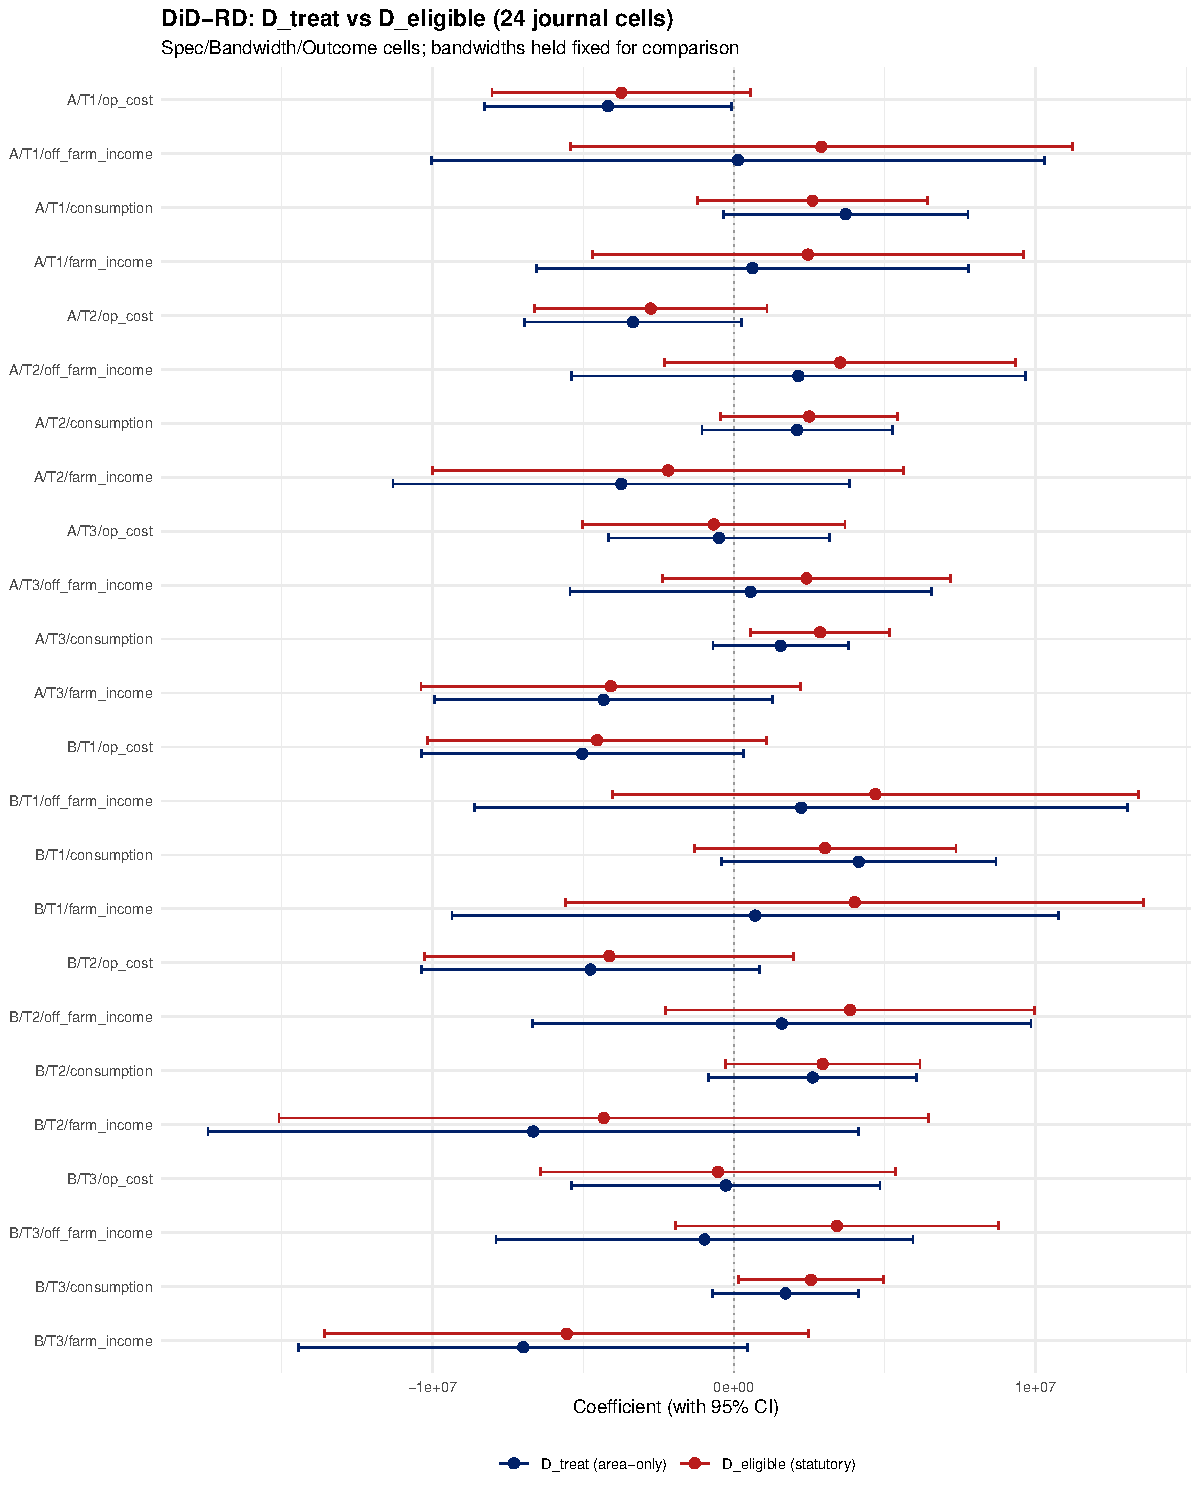
\includegraphics[width=0.80\textwidth]{../../scripts/R/_outputs_symmetric/fig_forest_treatment_definitions_en.pdf}
\caption{면적 단독 기준선 $D^{\text{area}}_i$(파란색)와 대칭 스크리닝 주 설계 $D_i$(빨간색)를 비교하는 24-저널-셀 계수의 forest plot. 헤드라인 F1 단조 임차율 구배와 음의 임차료 차감 영업비 방향은 두 처치 정의 모두에서 보존된다; 중위 절대 백분율 이동은 약 $39\%$이며 1개 부호 반전(농외소득, 두 설계 모두에서 풀링된 계수가 0에 가까움)과 $\alpha = .05$를 교차하는 3개 셀이 있다. 정성적 판독은 변경되지 않는다.}
\label{fig:forest-treatment-defs}
\end{figure}

\paragraph{Triple 자격 마진 조작 검정 (비대칭 표본 비교군).}\label{sec:robustness-multirv} 3개 FHES-관측가능 SFFP 자격 기준(i, ii, vi; \S\ref{sec:institutional-eligibility})은 각각 고유한 임계값을 가진 3개 실행변수를 생성한다. 주 설계(\S\ref{sec:identification})로 채택된 대칭 관측가능 자격 스크리닝 하에서, (ii)와 (vi) 마진은 각각의 임계값 양쪽에서 표본에서 조건화되어 빠지므로 그 두 마진에서의 McCrary 밀도 검정은 기계적이다(구성상 임계값 위 밀도가 0). 제도적 완전성을 위해 triple-margin 검정을 상위-꼬리 통제 가구를 유지하는 더 넓은 비대칭 표본 코호트에서 비교군으로 보고한다: 경지면적 임계값($5{,}000$\,m\textsuperscript{2}) 검정 통계량은 $t = 1.34$ ($p = .18$, $n = 2{,}680$); 자작 농지 임계값($15{,}500$\,m\textsuperscript{2})은 $t = -1.64$ ($p = .10$); 가구 농외소득 임계값(4,500만 원)은 $t = 0.18$ ($p = .86$). 세 마진 모두 이 비교군 패널에서 통상적인 수준에서 밀도-연속성 검정을 통과한다. 그림~\ref{fig:mccrary-multi-rv}은 임계값이 표시된 3개 기준 밀도를 시각화한다.

\begin{figure}[ht]
\centering
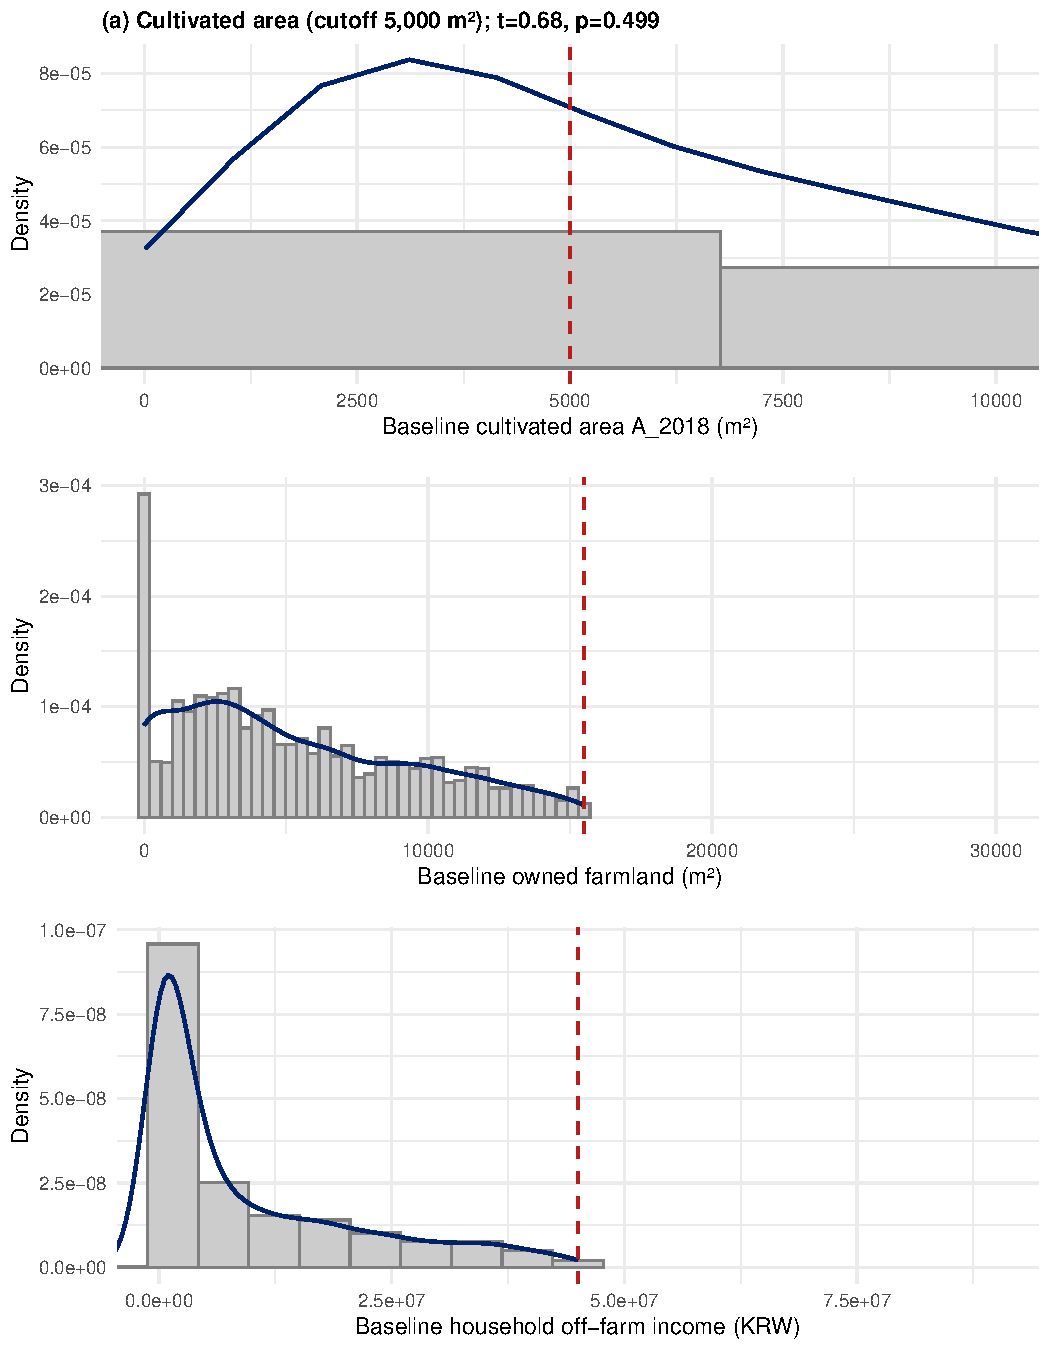
\includegraphics[width=0.78\textwidth]{../../scripts/R/_outputs_symmetric/fig_mccrary_multi_rv_en.pdf}
\caption{Triple 자격 마진 조작 검정. 각 패널은 하나의 FHES-관측가능 SFFP-자격 실행변수의 기준(2018) 밀도를 보여주며, 법정 임계값은 빨간 점선으로 표시. McCrary 2008 t-통계량: 경지면적 $t=1.34$ ($p=.18$); 자작 농지 $t=-1.64$ ($p=.10$); 가구 농외소득 $t=0.18$ ($p=.86$). 세 마진 중 어느 것도 통상적 수준에서 통계적으로 유의한 밀도 불연속을 보이지 않는다.}
\label{fig:mccrary-multi-rv}
\end{figure}

% =============================================================================
\section{논의 및 결론}
\label{sec:discussion}
% =============================================================================

\paragraph{정책적 함의.} SFFP의 농가별 정액 설계는 0.5\,ha 컷오프에서 신용제약 비-순소유 소농 부분모집단 내에 실질적으로 의미 있는 토지-보유 이동을 유도한다. T2에서의 순임차 자작면적 반응 $+1{,}151$\,m\textsuperscript{2}은 0.5\,ha 자격 임계값의 약 23\%이며, 동일한 반응이 4개 비-순소유 임차율 구간에 걸쳐 단조 감쇠한다($+1{,}151 \to +438 \to +258 \to -52 \to 0$). 이 패턴은 낮은 기준 자작비율을 가진 가구 사이에서 완화된 임차-자작 마진과 연관되며, 자산편향 유동성 메커니즘과 일치한다. 좁은 대역폭에서의 임차료 차감 영업비 반응(T1에서 $-3.57$\,M\,KRW)은 부담-받는 검정이 아니라 (\ref{eq:CO-3})의 (S,s) 비활동 예측을 지지한다: $T_{SFFP}/\tau \in [0.024, 0.048]$에서 이전소득은 불연속 자본조정 교차를 촉발하기에 너무 작으며, 가구는 한계 보조금을 덩어리 자본 스톡 확장이 아닌 변동비 마진에서 흡수한다.

\paragraph{Kirwan(2009)과 Baldoni-Ciaian(2023)과의 귀착 반전 대비.} T1에서 $-13.7\%$($p < .10$)와 T2에서 $-11.7\%$의 축약형 임차료 전가는 미국 농무부 직접 지급에 대해 \citet{Kirwan2009_rentcap}이 관찰한 $+25\%$ 지주 임차료 자본화와 EU 공동농업정책 1축에 대해 \citet{BaldoniCiaian2023_eucap}이 보고한 $+46$--$55\%$ 단기 / 장기 전가를 반전시킨다. 귀착 반전 뒤의 메커니즘은 농가별 정액 설계 자체이다: SFFP 자격은 지주가 임대 재협상을 통해 추출할 수 있는 한계 ha당 지급이 아니라 이진 가구-수준 처치이다. 음의 축약형 $\hat\beta_5$는 가구 수준 임차면적 대체에서 자작으로의 집계 평형 함의이다: 농가-모형 핵심은 $\hat\beta_5$를 직접 예측하지 않지만 관측된 임대-시장 반응으로 집계되는 기저 면적-대체를 생성한다. 표준 귀착 이론 \citep{Floyd1965_incidence, AlstonJames2002_incidence}은 감소된 임대수요 일정(자격 소농이 임차에서 자작으로 대체할 때 축소됨)을 음의 평형-임대료 반응에 매핑한다; $\hat\beta_5$는 모형의 경험적 footprint와 일치하는 축약형 증거로 보고되며, 일차 이론적 기여로 보고되지 않는다.

\paragraph{한국 소농 맥락.} 0.5\,ha 컷오프에서 관찰되는 신용제약 소농 코호트는 고령 운영자 모집단(세대주 평균 연령 약 67세; 재현 패키지 descriptives 표 참조), 논벼 생산(경지면적의 약 85\%), 처치 농가 중 52\% 순소유 비율에 의해 지배된다(자산편향 메커니즘은 F1 4-구간 구배에 따라 48\% 비-순소유 마진에서 작동한다). 자격 농가의 92.3\% 행정-수령률은 높은 정책 가시성을 반영한다; 본 연구의 DiD-RD 설계에서 imputation-추동 100\% ITT coverage는 AHM-확장 검정에 대한 적절한 식별 표적이다. 이 결과가 면적당 지주-포착 채널을 단절하는 다른 소규모-농장 직불금 설계로 확장되는지 여부는 열린 질문이다; 농가별 정액 이전소득에 관한 더 넓은 아시아-소농 문헌은 별도 식별을 조건으로 이 귀착 반전을 설계-추동 가능성으로 생산적으로 고려할 수 있다.

\paragraph{인구통계학적-도구변수 분리성 검정에 대한 보완.} 분리성 검정 문헌 \citep{Benjamin1992_separation, LaFaveThomas2016_markets}은 일반적으로 개발도상국 환경(예: 인도네시아, 인도)에서 구조적 검정을 위해 인구통계학적 충격(가구 구성)을 도구변수로 사용하여 분리성을 기각해 왔다. 본 연구의 환경은 두 방향에서 이 문헌을 연결한다. 첫째, 선진국 환경(한국, OECD 고소득 경제)에서 분리성을 기각하여, AHM-분리성 귀무가 신용 및 노동시장이 명목상 잘 발달된 곳에서도 실패할 수 있음을 증명한다. 둘째, 인구통계학적 도구변수가 아닌 sharp 정책 컷오프를 식별에 사용하여, 도구변수-배제-제한 위반과 가구-구성 내생성에 관한 전형적 우려를 제거한다. 공유된 실질적 판독---신용, 노동, 또는 토지시장이 소농 마진에서 불완전할 때 분리성이 실패함---은 두 식별 전략에 걸쳐 강건하다.

\paragraph{한계.} 세 가지 caveat가 헤드라인을 누그러뜨린다. (i) DiD-RD 설계는 단일 사전기간(2018$\to$2019)을 사용하며, \citet{Roth2022_pretrends}에 따라 사전추세 추론을 제한한다; 선형-추세-편향 강건성을 정량화하기 위해 \citet{RambachanRoth2023_honestdid} $\bar M$ 민감도 한계를 보고한다(\S\ref{sec:robustness}). (ii) FHES 1차 패널은 분석 윈도우를 2018--2022로 제한한다; 2차 마이크로데이터 linkage(2023년 이후)은 다가오며 Carter-Olinto 임계값 규칙의 장기 동적 확장을 가능하게 할 것이다. (iii) F2 감독-채널 계수 $\hat\beta_4$는 대역폭에 걸쳐 통계적으로 0에 가깝지만, EK 도출의 부호-비결정성(\S\ref{sec:supervision})은 깨끗한 해석을 방해한다: null은 SFFP 규모에서 감독 wedge가 slack한 것이나 상반된 가족-시간과 현금-제약 효과가 정확히 상쇄되는 것과 관측적으로 등가이다. 0.5\,ha 컷오프는 제도적으로 고유하다; 다른 한국 정책 임계값이나 다른 아시아 소농 맥락으로의 외부 타당성은 별도 연구를 요구한다---대안 비-분리성 문헌(\citealp{BanerjeeGertlerGhatak2002_tenancy}의 임차 계약 설계; \citealp{KhanThomas2008_idiosyncratic}의 거시 투자 이질성)에 대한 한 줄 참조는 범위 외이지만 관련된 비교 대상으로 제공된다.

\paragraph{결론.}\label{sec:conclusion}
한국의 농가별 정액 소농직불금의 0.5\,ha 자격 컷오프에서 농가모형의 분리성 귀무가설을 검정하고, \citet{CarterOlinto2003_liquidity}의 자산편향 유동성 채널을 통해 신용제약 비-순소유 부분모집단에 대해 이를 기각한다. T2에서의 순임차 자작면적 반응 $+1{,}151$\,m\textsuperscript{2}($p = .036$)과 단조 4-구간 임차율 구배(pure\_tenant, low\_owner, mixed, high\_owner, pure\_owner에 걸친 $1{,}151 \to 438 \to 258 \to -52 \to 0$)은 자산편향 시그너처를 고유하게 식별하며, 모든 부분집단이 비례적으로 반응할 보편적 소득효과 채널을 배제한다. T1에서의 임차료 차감 영업비 반응 $-3.57$\,M\,KRW는 보정된 $T_{SFFP}/\tau \in [0.024, 0.048]$에서 (S,s) 비활동 판독을 지지하지만, 개별적으로 유의하지 않다. T1에서의 $-13.7\%$ 임차료 전가($p < .10$)는 자작으로의 가구 수준 면적-대체의 집계 평형 함의로 보고된다; 면적비례 미국·EU CAP 설계 하에서 관찰된 $+25\%$--$55\%$ 지주 임차료 자본화를 반전시키며, 농가별 정액 메커니즘이 지주-포착 채널을 단절하는 것과 일치한다.

0.5\,ha SFFP 컷오프는 식별 도구로서 중요하다: 동결된 2018-기준 실행변수는 구성상 정책 후 조작을 배제하며, 농가별 정액 설계는 지주 임대료 추출을 제거한다---인구통계학적-도구변수 접근법 \citep{Benjamin1992_separation, LaFaveThomas2016_markets}이 깨끗하게 분리할 수 없는 confound이다. 결과는 대칭 스크리닝 부분모집단에 대한 불연속 기반 ITT 식별을 통해 선진국 소농 환경으로 분리성 검정 문헌을 일반화하며, 4-구간 임차율 구배는 보편적-소득-효과 대안이 일치시킬 수 없는 구조적으로 해석 가능한 시그너처를 제공한다.

향후 연구를 위해 네 가지 방향이 열려 있다. (i) 본 연구의 명세에서 농외소득 감독-채널 계수 $\hat\beta_4$는 0에 가깝다; 더 풍부한 한국 노동시장 자료---특히 2023년 이후 공개로 예정된 FHES 2차 linkage---는 상쇄-regime 대안을 slack-wedge 대안에서 분리함으로써 Eswaran-Kotwal(1986) 감독비용 메커니즘에 대한 더 정교한 검정을 가능하게 할 것이다. (ii) Carter-Olinto 임계값 규칙은 현재 정적 2-기간 도출이다; 다년 동적 확장---2020--2030 horizon에 걸쳐 자산 축적과 보유 전환을 추적---은 SFFP에 의해 유도된 중기 토지-보유 궤적에 대한 예측을 생성할 것이다. (iii) 한국농경제학회(KAEA) 및 KAEA-관련 저널을 표적으로 하는 paper/ko 한국어판이 대기 중이다; 한국어 초안은 학위논문 chapter 버전의 기반으로 사용될 것이다. (iv) 한국이 SFFP-자격 모집단을 확장하기 위해 두 번째 농가별 정액 자격 임계값(예: 1.0\,ha)을 도입한다면, 컷오프 간 재현은 채널-상대-magnitude를 더 정확히 식별하고 자산편향 시그너처가 다른 소농 규모에서 지속되는지 검정할 것이다.

% =============================================================================

\bibliography{../../Bibliography_base}

\end{document}
